%%%%%%%%%%%%%%%%%%%%%%%%%%%%%%%%%%%%%%%%%%%%
\chapter{Results}
%
\begin{center}
  \begin{minipage}{0.75\textwidth}
    \begin{small}
      “I hear and I forget. I see and I remember. I do and I understand”\\
      \null\hfill\emph{Confucius}
    \end{small}
  \end{minipage}
  \vspace{0.5cm}
\end{center}
\section{Optimization of Parameters}
The histograms that resulted from measuring the S1 and S2 polarization showed evidence of masking and shadowing effects due to macro level surface features.  This caused some pixels to never be illuminated and have a large spike at zero.

Pixels that were never illuminated were removed from the histogram process. These were determined by checking if $P_H, P_V, P_P$, and $P_M$ never had a value more than 0.  This removed the spike at zero.

The free parameters in Support Vector Classification were optimized using the Sklearn grid search module.

%%%%%%%%%%%%%%%%%%%%%%%%%%%%%%%%%%%%%%%%%%%%%
\section{Classification}
%%%%%%%%%%%%%%%%%%%%%%%%%%%%%%%%%%%%%%%%%%%%%
Images were acquired for each polarization filter orientation. Red Oak, American Ash, and Sugar Maple leaves were measured immediately after being removed from their host tree and polarization measurements were recorded.  The same procedure was then performed 1 week later.  These measurements produce interclass variance and show the effects of the decomposition process on the polarization response and texture of various leaf species.  In total 18 different leaves were investigated for classification purposes under experimental design setup 1.  Images were acquired in both the specular and diffuse directions for each leaf.  100 samples of 75 by 75 pixels were extracted from each leaf to represent various textures found on the surface and the physiological status below the surface.  In total 1800 samples were used to perform classification and validation using a linear support vector classifier.
%%%%%%%%%%%%%%%%%%%%%%%%%%%%%%%%%%%%%%%%%%%%%%
\subsection{Specular Leaves}
%%%%%%%%%%%%%%%%%%%%%%%%%%%%%%%%%%%%%%%%%%%%%%
%
\begin{figure}[htp]
    \centering
    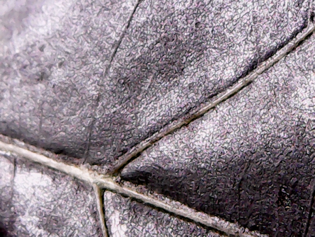
\includegraphics[width=.3\textwidth]{/Sources/Results/721/oak-raw.png}\hfill
    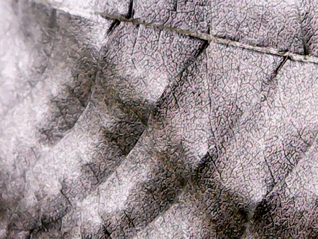
\includegraphics[width=.3\textwidth]{/Sources/Results/721/Ash-raw.png}\hfill
    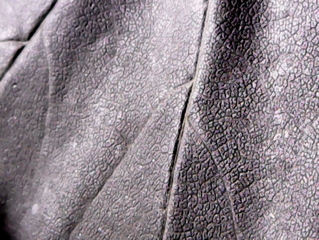
\includegraphics[width=.3\textwidth]{/Sources/Results/721/sugar-raw.png}

    \caption{From left to right: Red Oak, American Ash, and Sugar Maple through H polarization filter in the Specular Direction.}
    \label{fig:specular-raw}
\end{figure}
%
The principles of reflection and transmission as dictated by Fresnel’s equations show that light reflecting from a specular surface will have higher amounts of polarization than when compared with the diffuse direction.  The S1 component for all leaves showed this response as expected and produced higher amounts of polarization than when compared to their diffuse counterparts.  The S2 component showed itself to have a near zero mean, with some variance.

The histograms for the S1 and S2 parameters comparing different tree leaves were computed for the blue, green and red camera channels.  These individual channels in general are the same as the overall grey level image shown as RGB here, although more distinguished features can be seen in Figure 7.2 for each individual channel.
%
\begin{sidewaysfigure}
    \begin{center}
        \makebox[\textwidth]{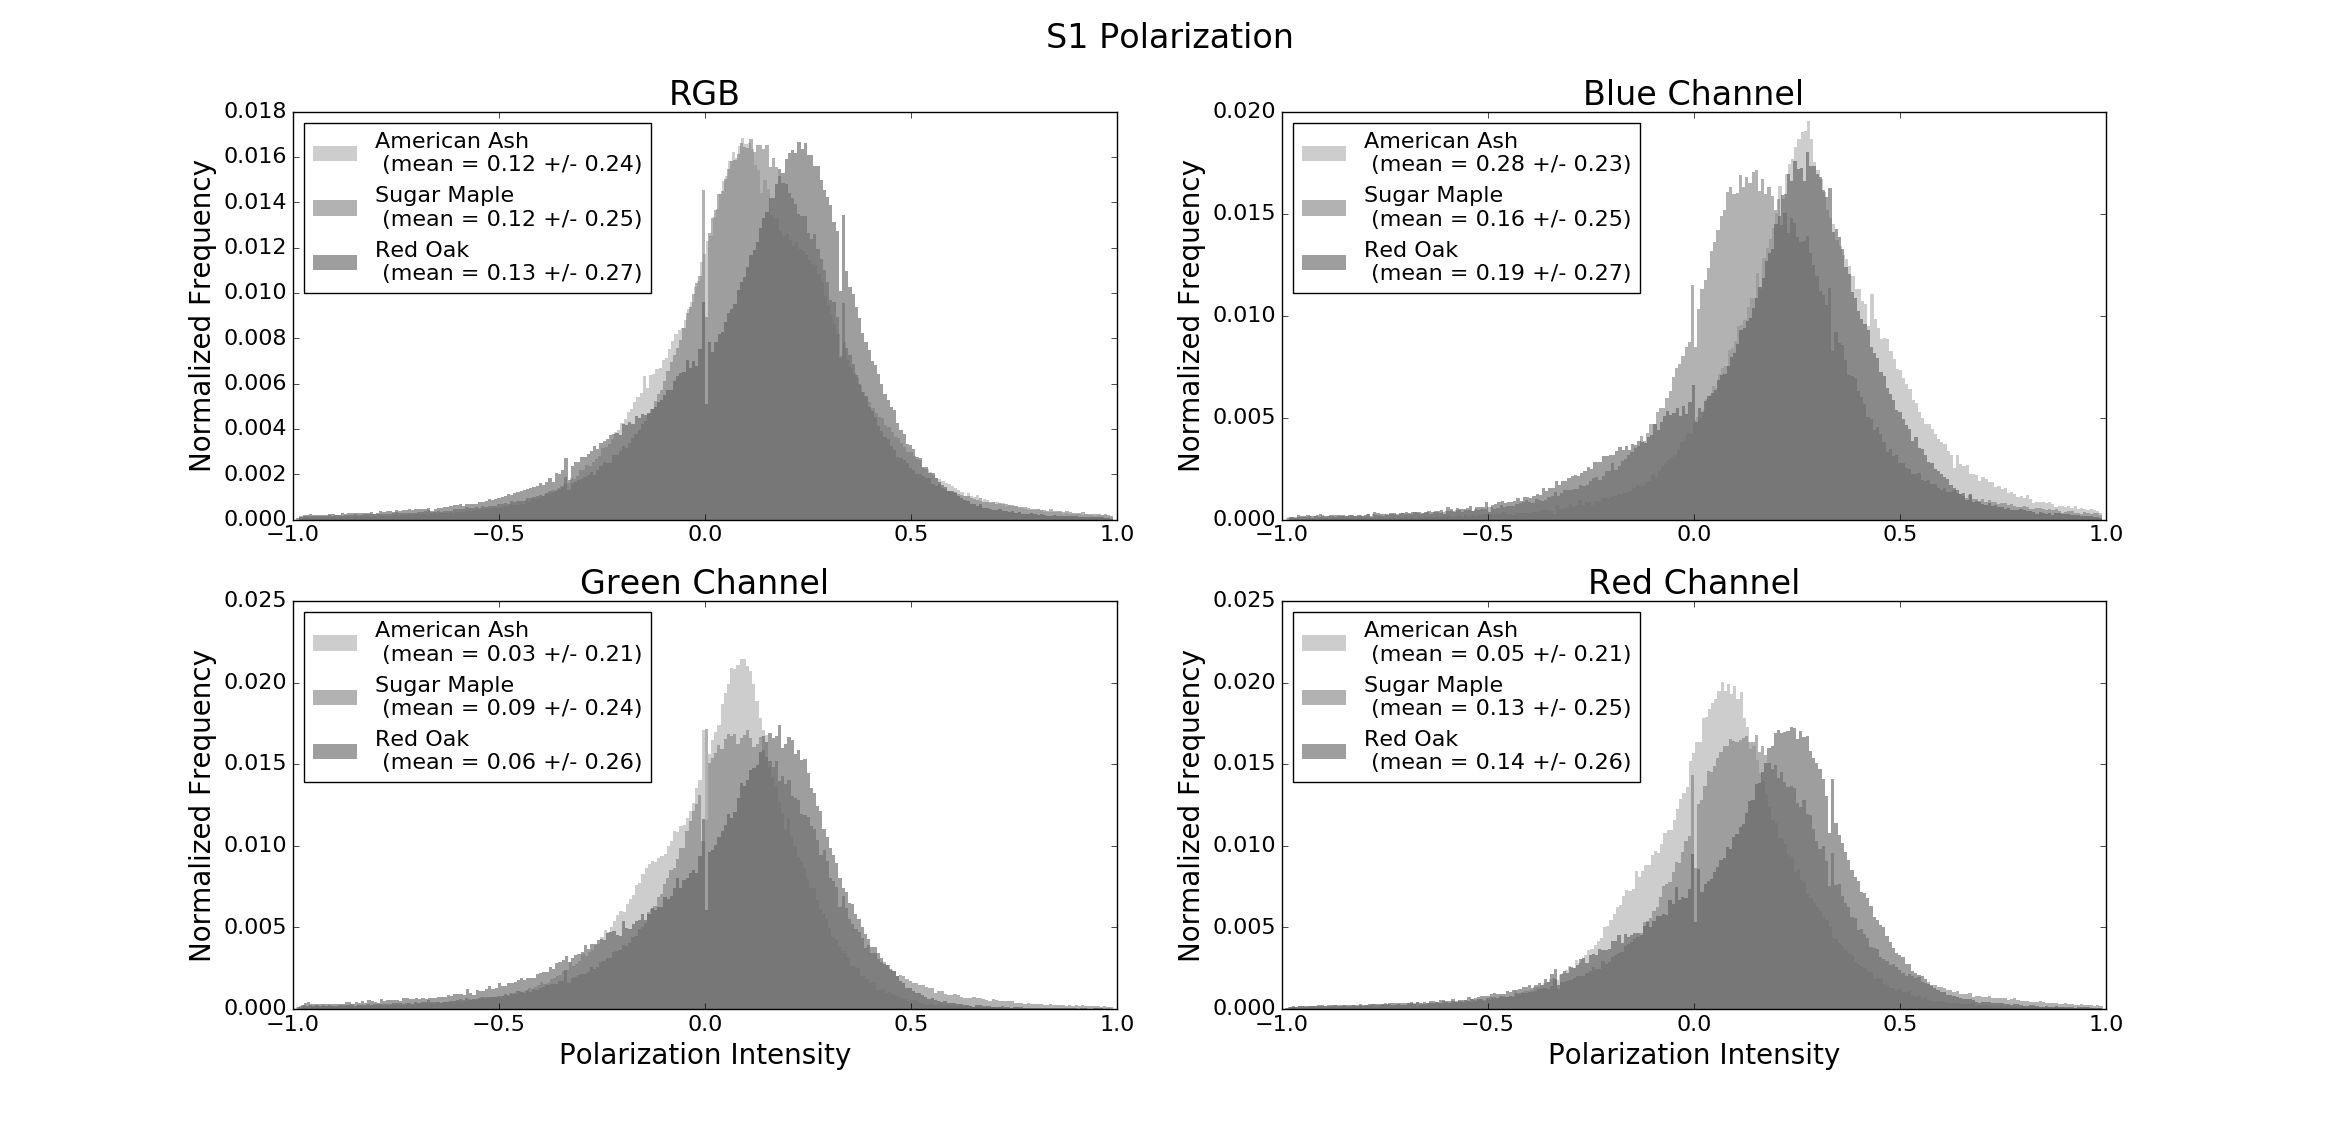
\includegraphics[scale=0.4]{/Sources/Results/721/allhistpolarization-v2.png}}
    \end{center}
    \caption{All plants specular observed direction for each RGB channelization 0 week for S1}
    \label{fig:polarization}
\end{sidewaysfigure}
%
%
The blue and red channel show higher amounts of polarization, while the green channel shows the least amount of polarization, across each species.  It has previously been shown, that Rayleigh scattering on a leafs' surface can greatly increase the polarization in the blue spectrum of light [26].  Since plants reflect highly in the green, the green channel shows the lowest amount of polarization.  The blue channel shows the most amount of polarization, although this may be due to the sensitivity of the CMOS sensor or Rayleigh scattering [26].  The blue channel is extended to regions of red light and therefore is overall more sensitive in the visible region to spectral fluctuations.  Perhaps in the future, the blue channel response should be subtracted from the red channel response, and the blue channel can be normalized using the following ratio,
%
\begin{align}
    Blue_{calibration} = Blue - (Blue - Red)
\end{align}
%
Ideally the response of each channel would be carefully calculated using a spectrometer, and overall constants could be provided to normalize the sensitivity in each spectral region.  This requires various narrow band spectral filters.

The S2 histograms in Figure 7.3 show very little polarization on average.  This is expected polarization angles at 45 and 135 can be decomposed into $x$ and $y$ components.  It is possible that the S2 component could be useful in understanding the calibration of the linear polarizer to its ideal orientation.  If P and M measurements diverge drastically, it would serve as a notion to investigate the variance further for specular reflections.
%
\begin{sidewaysfigure}
    \begin{center}
        \makebox[\textwidth]{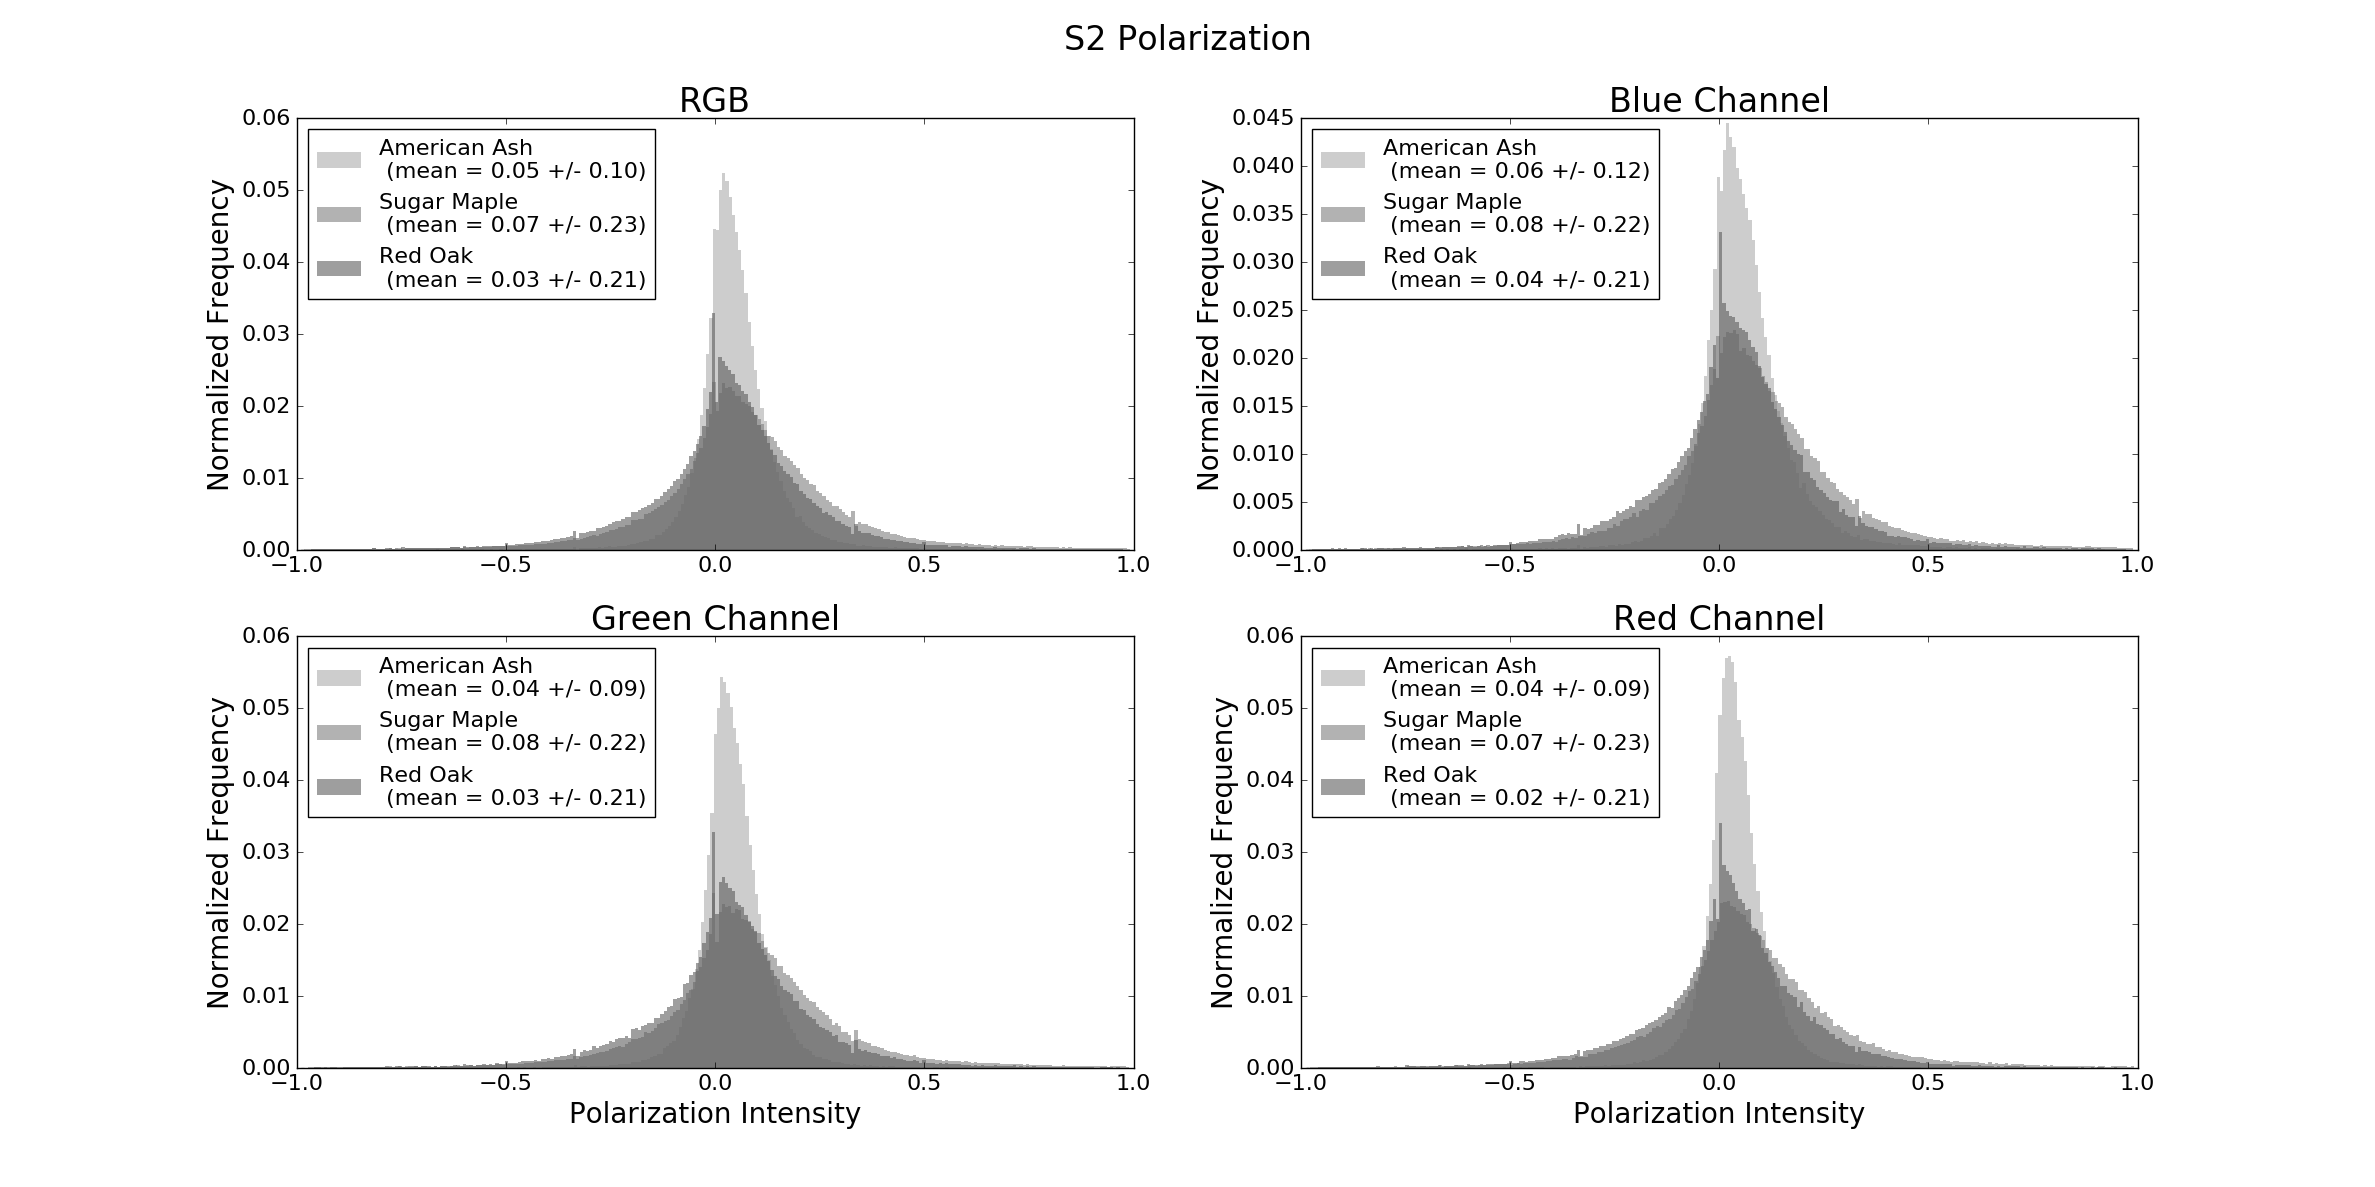
\includegraphics[scale=0.4]{/Sources/Results/721/all-s2-polarization-v2.png}}
    \end{center}
    \caption{All plants RGB channels observed from the specular direction 0 week for S2}
    \label{fig:polarization}
\end{sidewaysfigure}
The specular direction of observation and incident angle at the Brewster angle creates the highest amount of polarized light on an ideal smooth surface.  Leaves can also be seen to similarly have specular components that correlate to the surface topology.

A GLCM texture analysis was also performed on each sample extracted to determine the dissimilarity, contrast, entropy, and correlation. Due to each of the GLCM features being generated from the same initial matrix, many of the features show high levels of correlation.  In general, a measure should be taken from the orderliness group, contrast group and descriptive statistics group. It has been shown that a textures dissimilarity and correlation show low levels of correlation.  Therefore, they are plotted here to represent the texture in 2 dimensions.

Although these features contain information regarding the texture of a surface, it is often difficult to determine what actually causes each metric to arise when describing specific surface GLCM properties \cite{haralick}.

Figure 7.4 shows the texture of the leaves above for the V filter orientation.  It shows that each species exhibits its own unique texture that helps to visually create clusters, and therefore should prove useful for classification.
%
\begin{figure}
    \begin{center}
        \makebox[\textwidth]{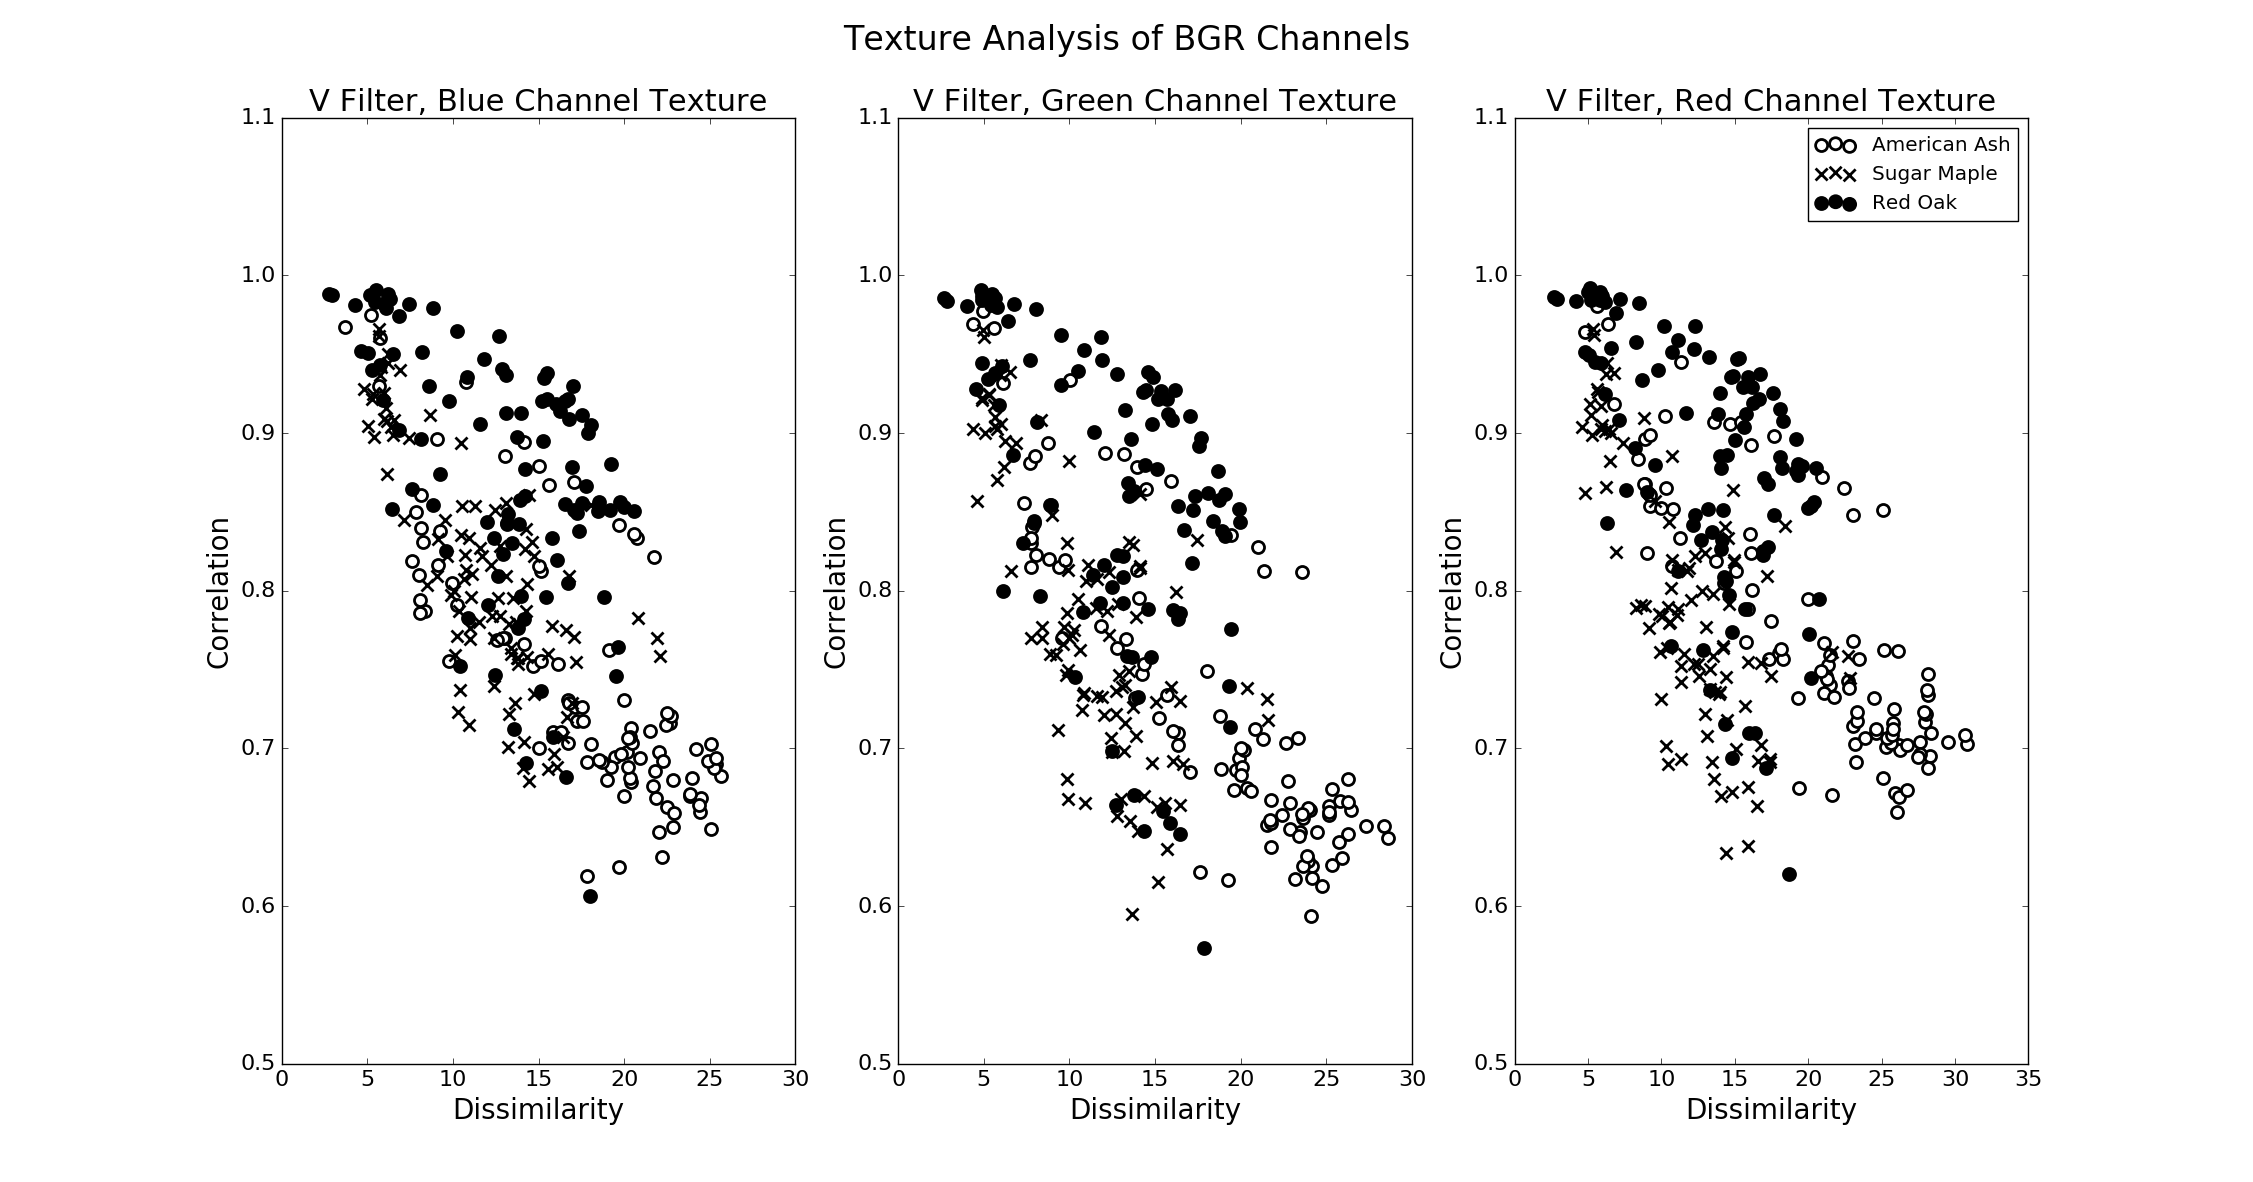
\includegraphics[scale=0.375]{/Sources/Results/glcm/specular/V-filter-all-species-rgb.png}}
    \end{center}
    \caption{V filter GLCM dissimilarity and correlation for all species in the specular direction week 0}
    \label{fig:polarization}
\end{figure}
%
Additional filter arrangements can be found in the Appendix.

\subsection{Specular Leaf Decomposition}
As leaves start to undergo pigment breakdown and decomposition, the surfaces of the leaves provide more reflectance.  The loss of water and pigment structure results in rougher external surface on the leaf that causes a more diffuse reflection, even when viewed at the Brewster angle.  This results in a loss of magnitude of S1 polarization as the leaf decomposes.  Visual changes to the surface of the leaf can be found in the original V filter images.
%
\begin{figure}[htp]
    \centering
    \hspace*{\fill}%
    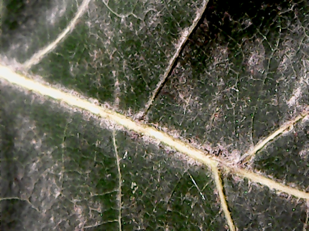
\includegraphics[width=.3\textwidth]{/Sources/Results/7_2_2/oak_new_raw.png}\hfill%
    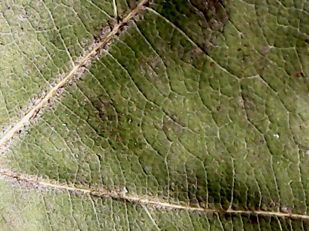
\includegraphics[width=.3\textwidth]{/Sources/Results/7_2_2/Oak_raw_1wk.png}
    \hspace*{\fill}%
    \caption{From left to right: Red Oak Freshly Removed and After One Week}
    \label{fig:specular-raw-decompose}
\end{figure}
%
Close inspection Figure 7.5 show that the new leaf is a darker green in color and has a smoother surface than the oak leaf after 1 week.  The smooth, thick wax surface as it ages from week 0 to week 1, becomes flatter and segmentation of structures on the leaf surface becomes more evident.

Recording the leaves after one week to illustrate changes during decomposition and water loss for red oak can be seen in Figure 7.6.  It should be noted that the blue channel contains a large amount of polarization after one week. In some cases, it has been seen to even exceed its 0-week counterpart. This may be due to the absorbance spectrum of chlorophyll and the lack of photosynthetic activity during decomposition. The overall S1 image shows the 0 week has higher polarization in S1 as its surface is more of a pure specular reflector.
%
\begin{sidewaysfigure}
    \begin{center}
        \makebox[\textwidth]{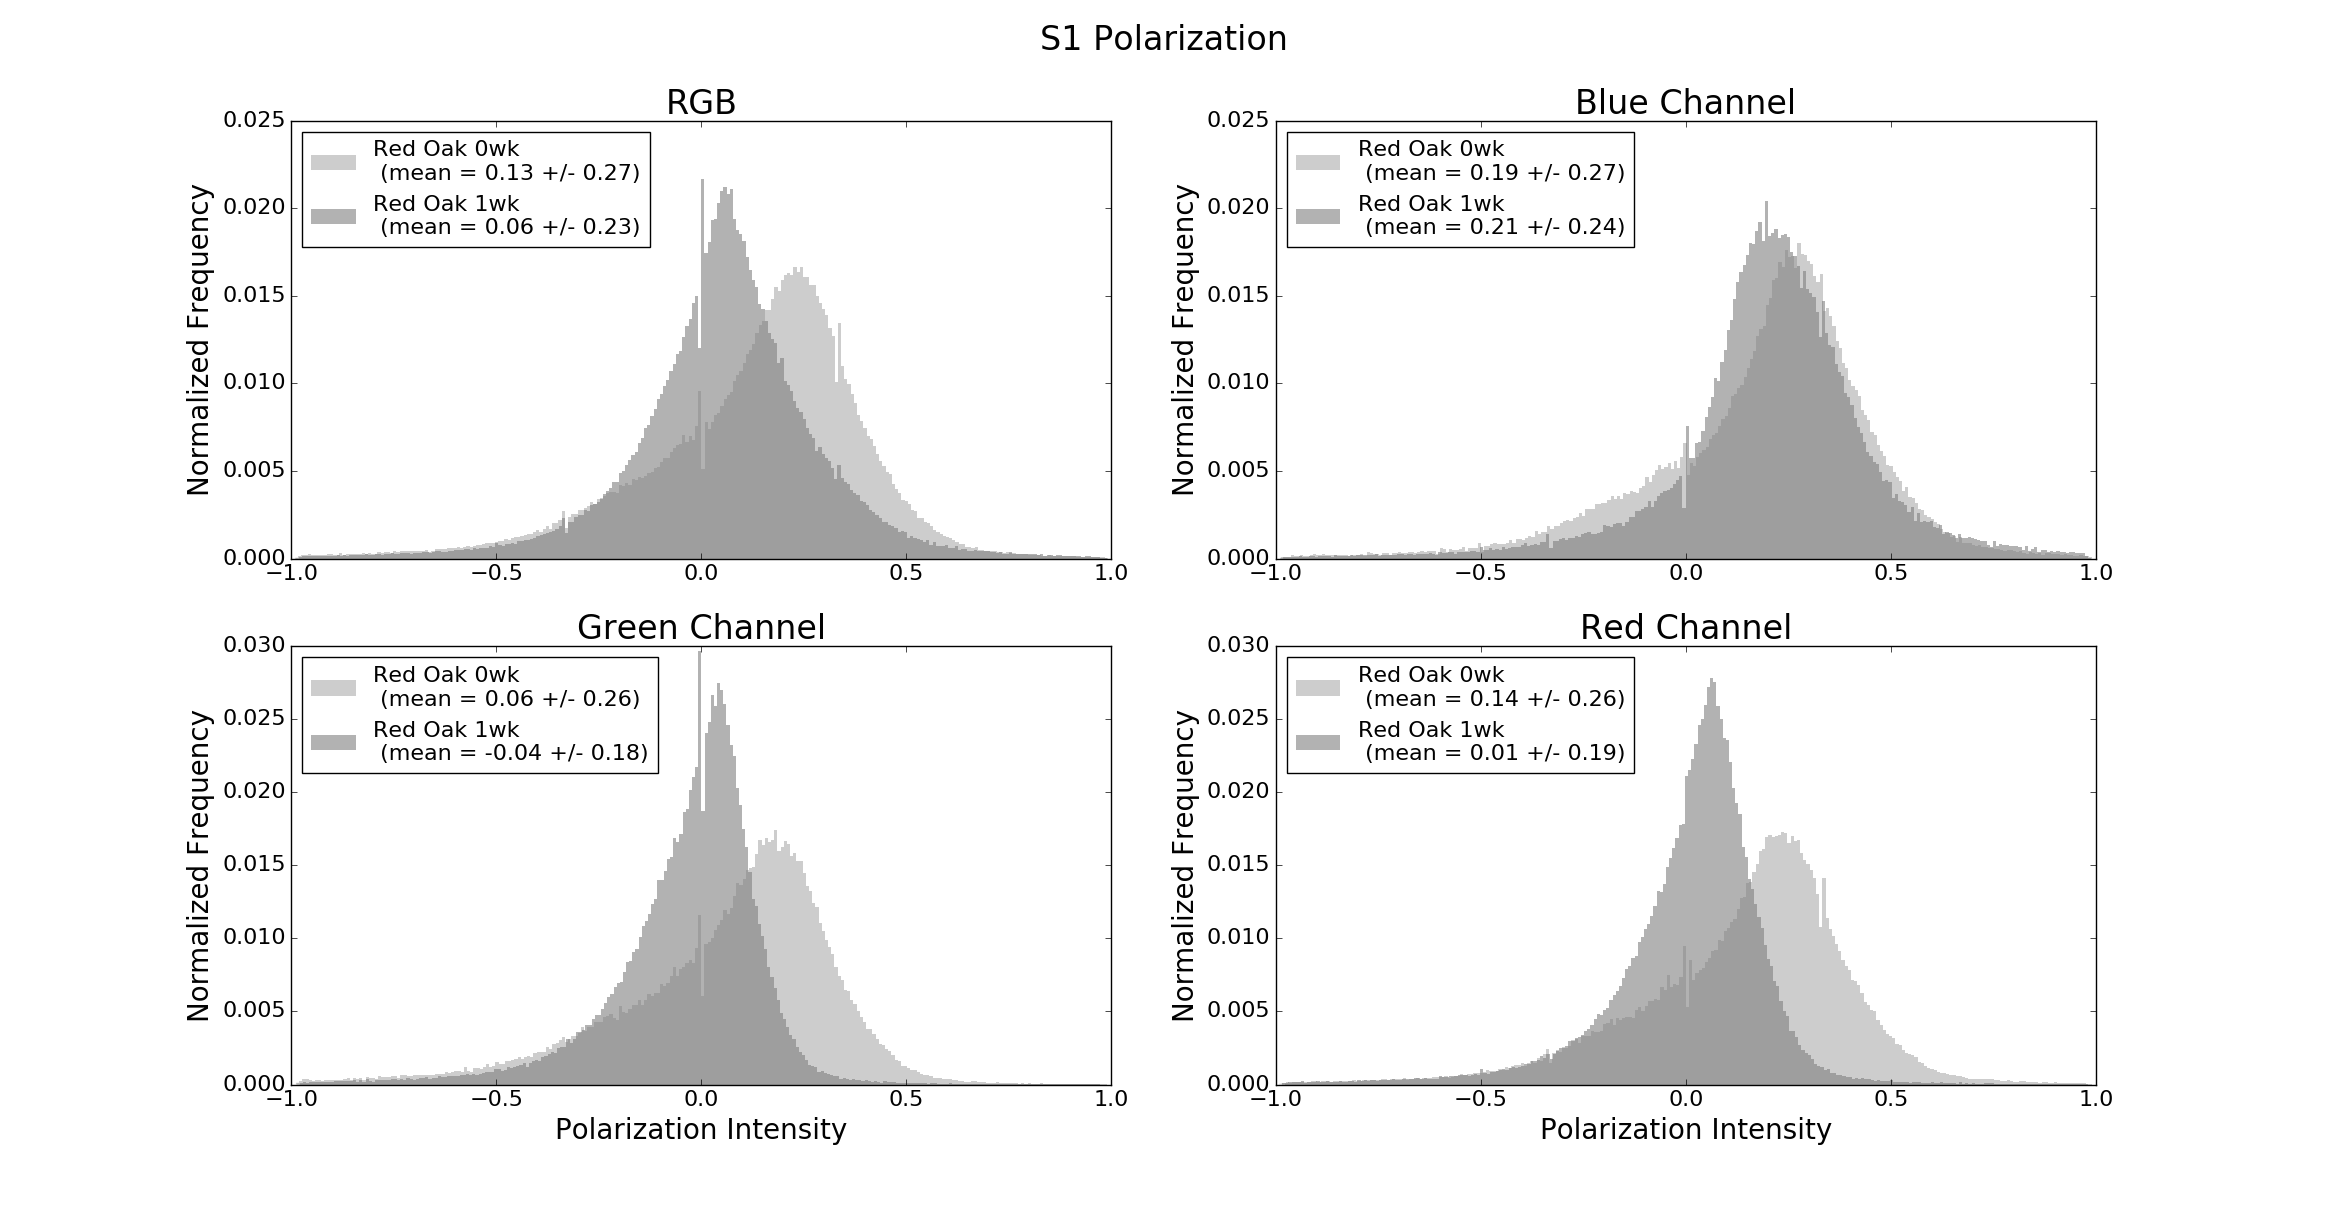
\includegraphics[scale=0.4]{/Sources/Results/7_2_2/S1_polar_v2.png}}
    \end{center}
    \caption{Red Oak 0 weeks and 1 week observed in the specular direction for S1}
    \label{fig:polarization}
\end{sidewaysfigure}
%
\begin{sidewaysfigure}
    \begin{center}
        \makebox[\textwidth]{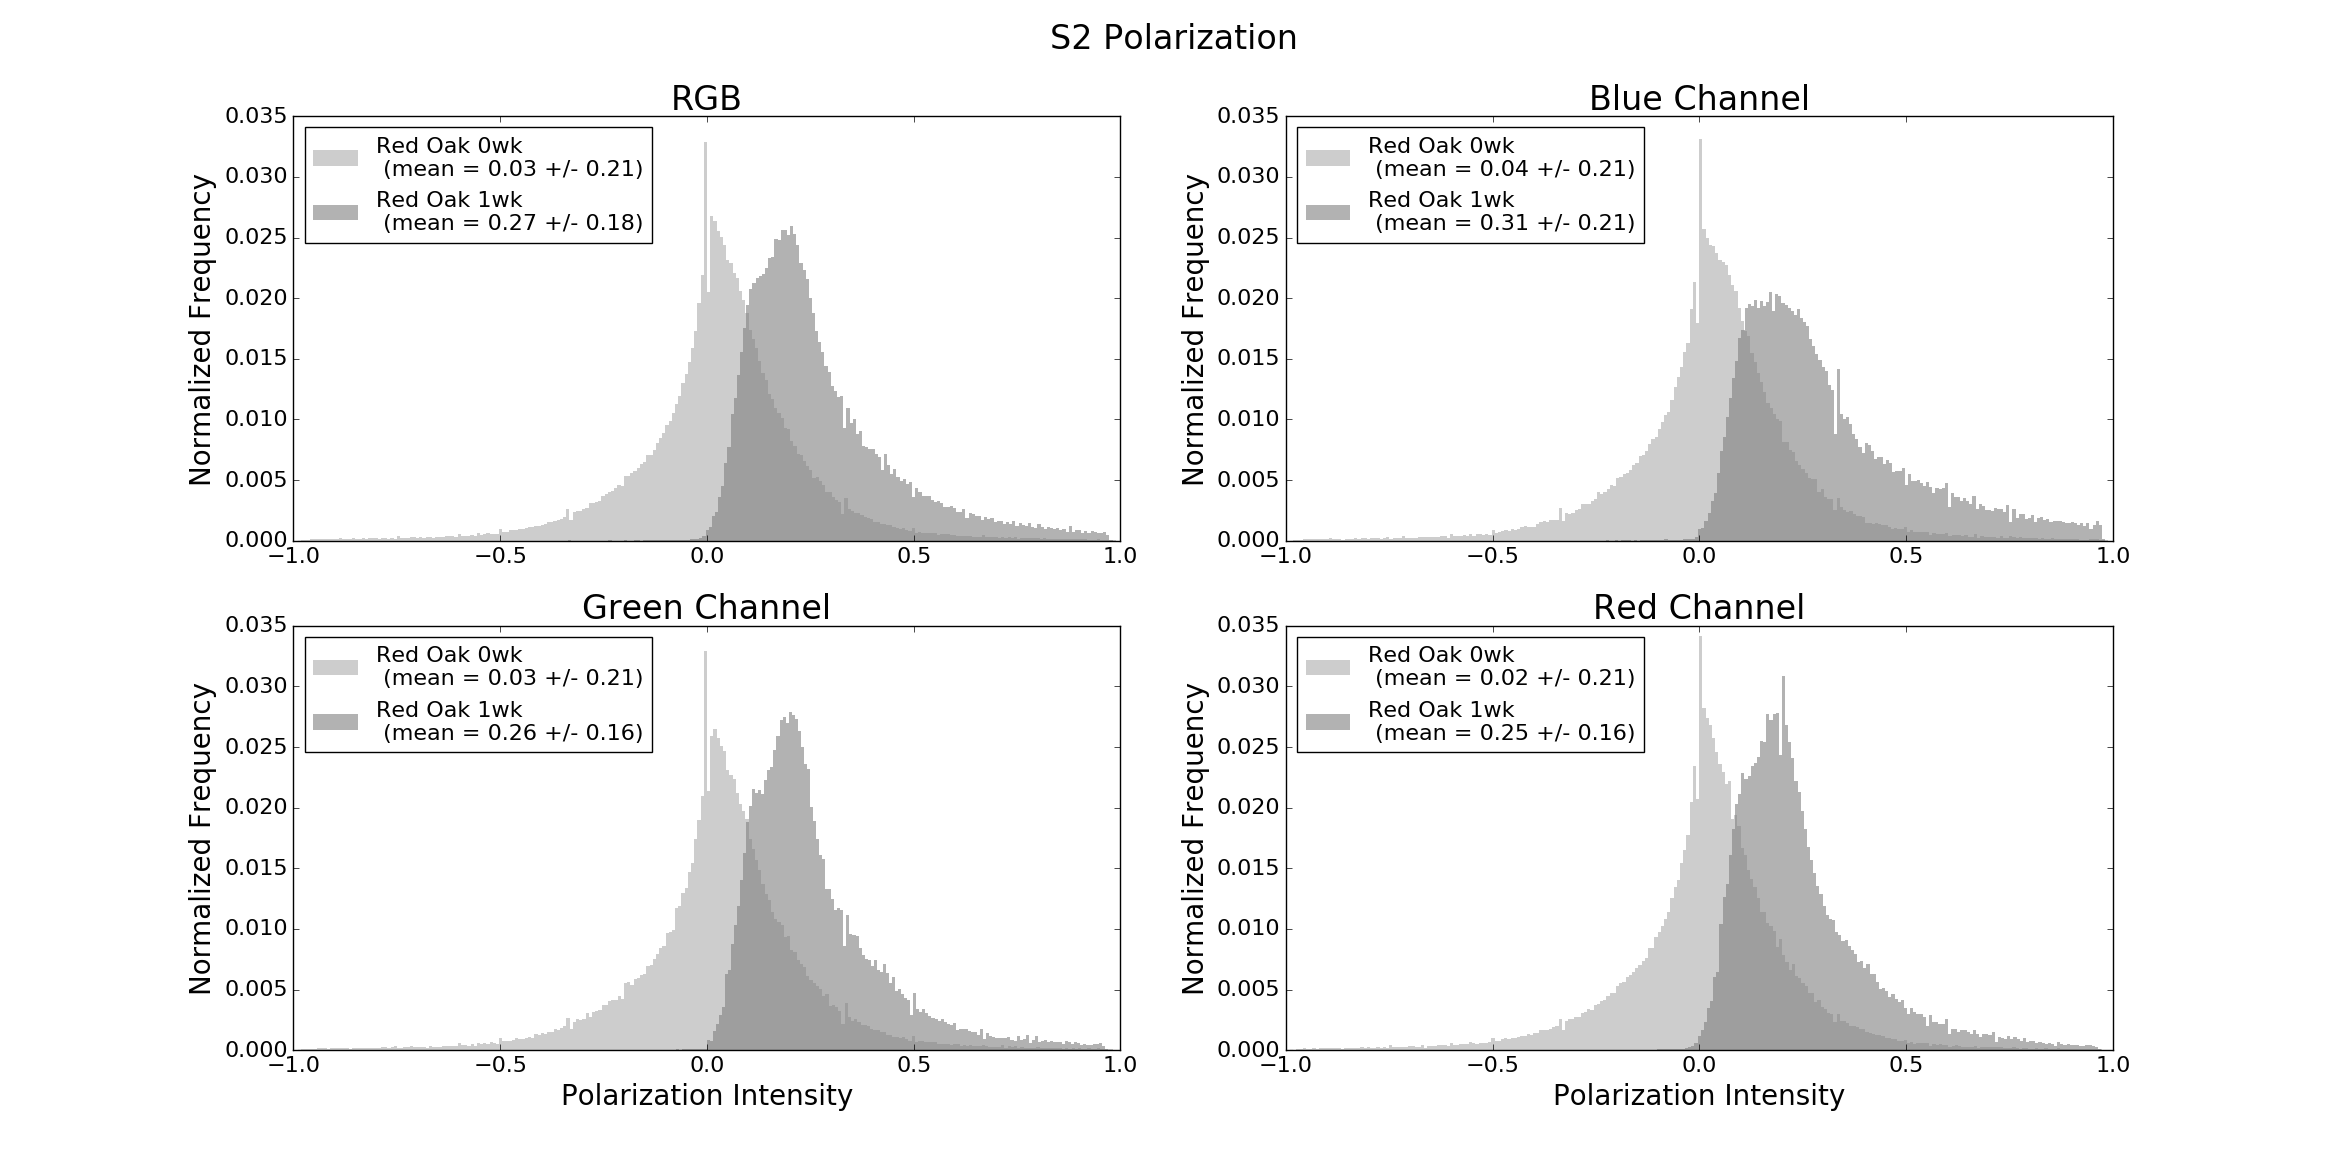
\includegraphics[scale=0.4]{/Sources/Results/7_2_2/S2_polar_v2.png}}
    \end{center}
    \caption{Red oak 0 weeks and 1 week observed in the specular direction for S2}
    \label{fig:polarization}
\end{sidewaysfigure}
%
Again S2 only shows a slight variation even after re-measuring the leaf one week later.

The results of GLCM analysis for the P filter component can be found in Figure 7.8.  Visual inspection of the GLCM scatter plot shows the best clustering using the P filter for this particular example.  The full GLCM filter set can be found in the Appendix.
%
\begin{figure}
    \begin{center}
        \makebox[\textwidth]{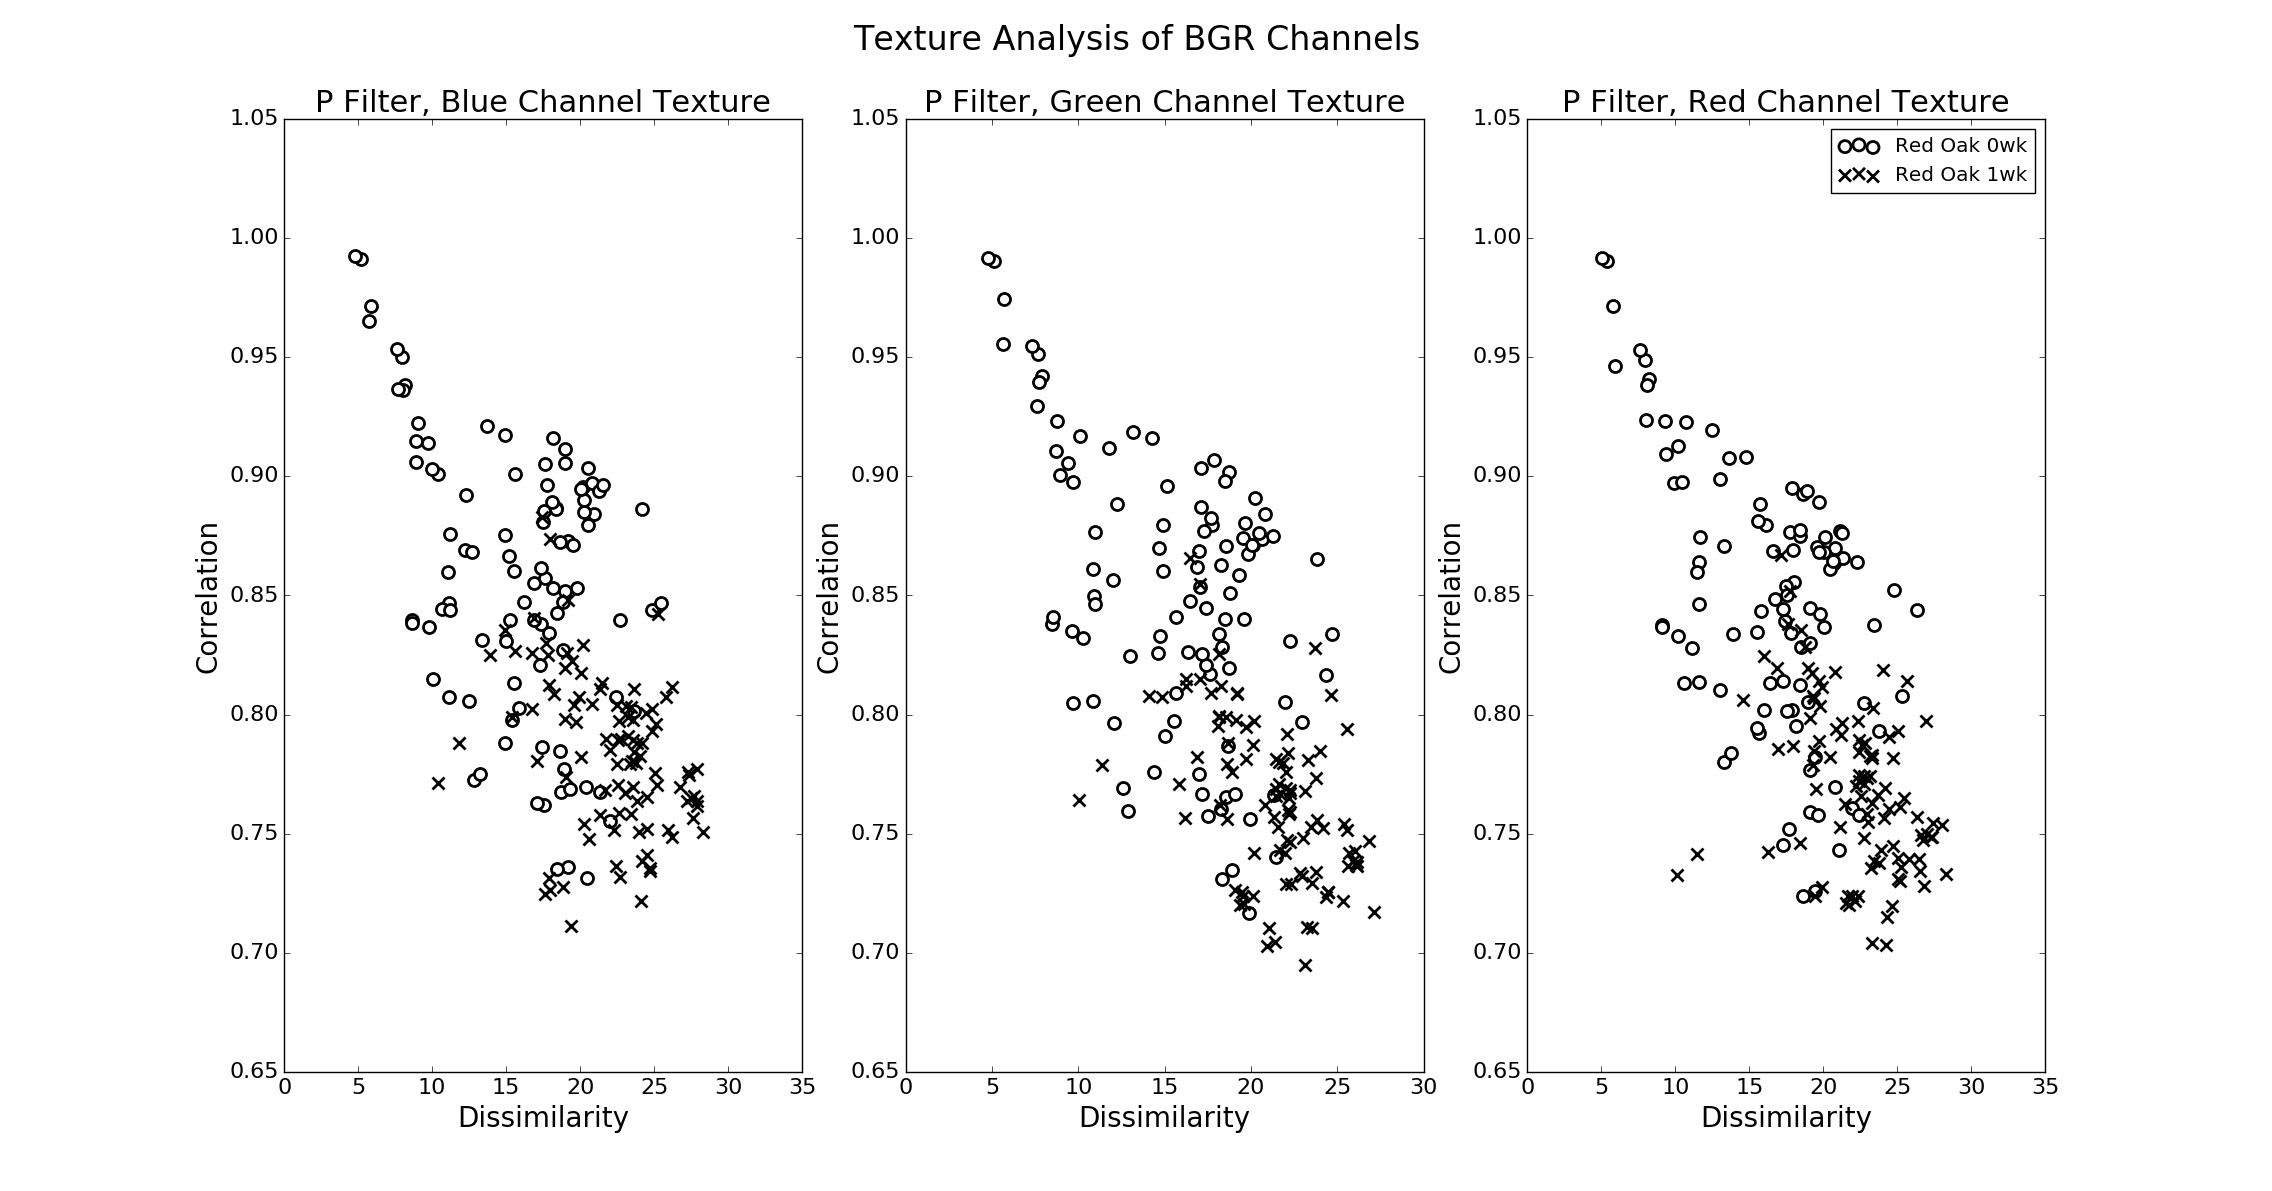
\includegraphics[scale=0.375]{/Sources/Results/glcm/specular/0wk-1wk-P-filter-red-oak-rgb-specular.png}}
    \end{center}
    \caption{P filter GLCM dissimilarity and correlation in specular direction for 0 and 1 week.}
    \label{fig:polarization}
\end{figure}
%
As water leaves the leaf which undergoes the decomposition process, the surface becomes rougher as the water that once supported much of the cells structure has been removed. The surface becomes more diffuse.  The highly specular component of healthy leaves, creates maximum intensity levels on the cameras detector, making the surface appear smooth.  This results in a higher amount of dissimilarity on the surface of the leaf after one week, as compared to one that is still healthy.  The correlation is shown to also decrease as a result of this process as well.

\subsection{Specular Classification Results}
Classification was performed on datasets created by combining texture samples from leaves that were both zero week and one week old.  This created variance within the classes themselves, as previously it has been shown how physiological changes within the leaf can lead to different polarization and texture results.  The results of classification show that there is still an ability to distinguish between species with a high amount of precision.

The confusion matrix also shows the high level of accuracy when using ten fold stratified K fold validation.  It can be seen that the highest accuracy of classification is when American ash is considered versus Maple or Oak.  Visual inspection of each type of leaf shows the similarity between Oak and Maple when viewed under a microscope, so this result is not unexpected.

A learning curve was also generated for the results of using both texture and polarization features and is shown in Figure 7.10.  As the number of training samples increases, the score of the classifier remains the same.  This shows the low amount of training bias within the model created from our samples. Future samples should be collected and compared to further validate these results.
%
\begin{figure}[!htb]
    \begin{center}
        \makebox[\textwidth]{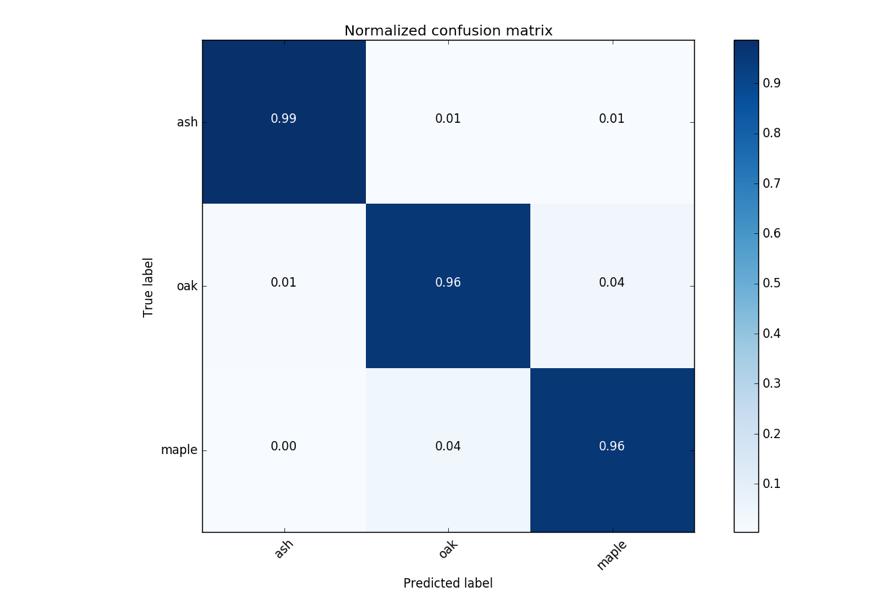
\includegraphics[scale=0.9]{/Sources/Results/7_2_3/confusion.png}}
    \end{center}
    \caption{Confusion Matrix for All Species observed in the specular direction.}
    \label{fig:polarization}
\end{figure}
%
%
\begin{figure}[!htb]
    \begin{center}
        \makebox[\textwidth]{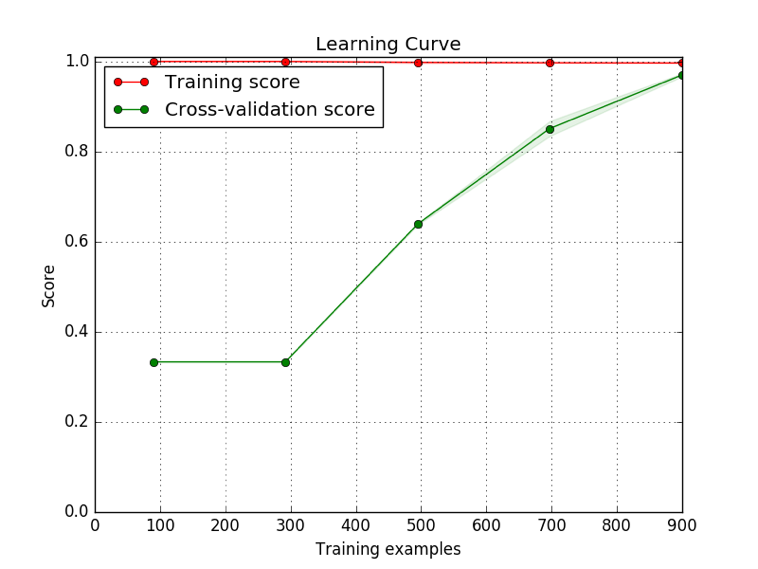
\includegraphics[scale=0.9]{/Sources/Results/7_2_3/learning_curve.png}}
    \end{center}
    \caption{Learning curve for leaves observed in the specular direction.}
    \label{fig:polarization}
\end{figure}
%
The overall results for specular classification for all species using polarization and texture features where class 0 is American Ash, class 1 is Red Oak, and class 2 is Sugar Maple.
%
\begin{table}[htb]
  \centering
  \begin{tabular}{lllll}
    \toprule
    \textbf{Class} & \textbf{Precision} & \textbf{Recall} & \textbf{F1 Score} & \textbf{Support} \\
    \midrule
      \texttt{0.0} & 0.99 & 0.98 & 0.99 & 600 \\
      \texttt{1.0} & 0.95 & 0.95 & 0.95 & 600 \\
      \texttt{2.0} & 0.96 & 0.96 & 0.96 & 600 \\
      \texttt{avg/total} & 0.97 & 0.97 & 0.97 & 1800 \\
    \bottomrule
  \end{tabular}
  \caption{%
    Scores for Classification in the Specular Direction with Polarization and Texture in Specular Direction.
  }
  \label{tab:Packages}
\end{table}
\begin{table}[htb]
  \centering
  \begin{tabular}{lllll}
    \toprule
    \textbf{Class} & \textbf{Precision} & \textbf{Recall} & \textbf{F1 Score} & Support\\
    \midrule
      \texttt{0.0} & 0.95 & 0.97 & 0.96 & 600 \\
      \texttt{1.0} & 0.88 & 0.92 & 0.90 & 600 \\
      \texttt{2.0} & 0.93 & 0.87 & 0.90 & 600 \\
      \texttt{avg/total} & 0.92 & 0.92 & 0.92 & 1800 \\
    \bottomrule
  \end{tabular}
  \caption{%
    Scores for Classification in the Specular Direction with Just Polarization in Specular Direction.
  }
  \label{tab:Packages}
\end{table}
%
\begin{table}[htb]
  \centering
  \begin{tabular}{lllll}
    \toprule
    \textbf{Class} & \textbf{Precision} & \textbf{Recall} & \textbf{F1 Score} & Support\\
    \midrule
      \texttt{0.0} & 0.97 & 0.96 & 0.96 & 600 \\
      \texttt{1.0} & 0.86 & 0.89 & 0.87 & 600 \\
      \texttt{2.0} & 0.90 & 0.87 & 0.88 & 600 \\
      \texttt{avg/total} & 0.91 & 0.91 & 0.91 & 1800 \\
    \bottomrule
  \end{tabular}
  \caption{%
    Scores for Classification in the Specular Direction with Just Texture in Specular Direction.
  }
  \label{tab:Packages}
\end{table}
%
It can be seen that combining both polarization and texture features for classification, results in better precision, recall, and F1 scores than if either of the feature sets are used independently.  This shows the benefit of using different types of features for classification.

\subsection{Diffuse Leaves}
%
\begin{figure}[htp]
    \centering
    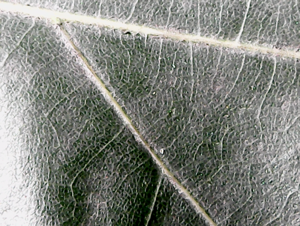
\includegraphics[width=.3\textwidth]{/Sources/Results/7_2_4/oak-raw.png}\hfill
    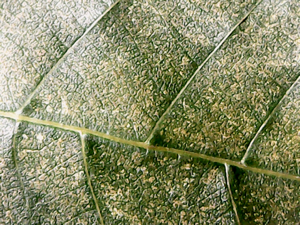
\includegraphics[width=.3\textwidth]{/Sources/Results/7_2_4/ash-raw.png}\hfill
    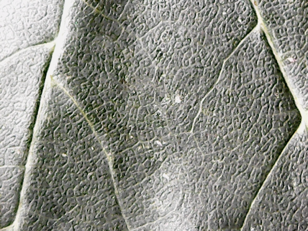
\includegraphics[width=.3\textwidth]{/Sources/Results/7_2_4/maple-raw.png}

    \caption{From left to right: Red Oak, American Ash, and Sugar Maple through H polarization filter in the Diffuse Direction.}
    \label{fig:specular-raw}
\end{figure}
%
Leaves from each species of tree were acquired at 0 degrees from the normal for the plane of incidence.  Examples of each leaf captured through the H filter can be found in Figure 7.11.

The diffuse component of reflectance of a leaf is often thought of as being unpolarized.  This assumption if based on a perfect Lambertian diffuse surface, which is often not the case.  Although the portion of polarized light in the diffuse region of reflection is less than that of the specular portion, it cannot be discarded, as it may contain important information as to the biological and physiological processes within the leaf's internal structure.

As photons undergo multiple scattering processes and absorption and reemission by chlorophyll, they can become partially or completely polarized.  These mechanisms are complex, and it is necessary to go beyond Fresnel’s equations to dictate the major processes at work in the diffuse component of scattering.  Polarimetric BRDF models attempt to ascertain the relationship between surface scatter and polarization of light.

Our results show that although the mean is centered around zero for S1, the S2 component shows various degrees of polarization.  These may be due to multiple scattering mechanisms within the layers of the leaf.

The diffuse portion of polarization for each species is shown in Figure 7.12.
%
\begin{sidewaysfigure}
    \begin{center}
        \makebox[\textwidth]{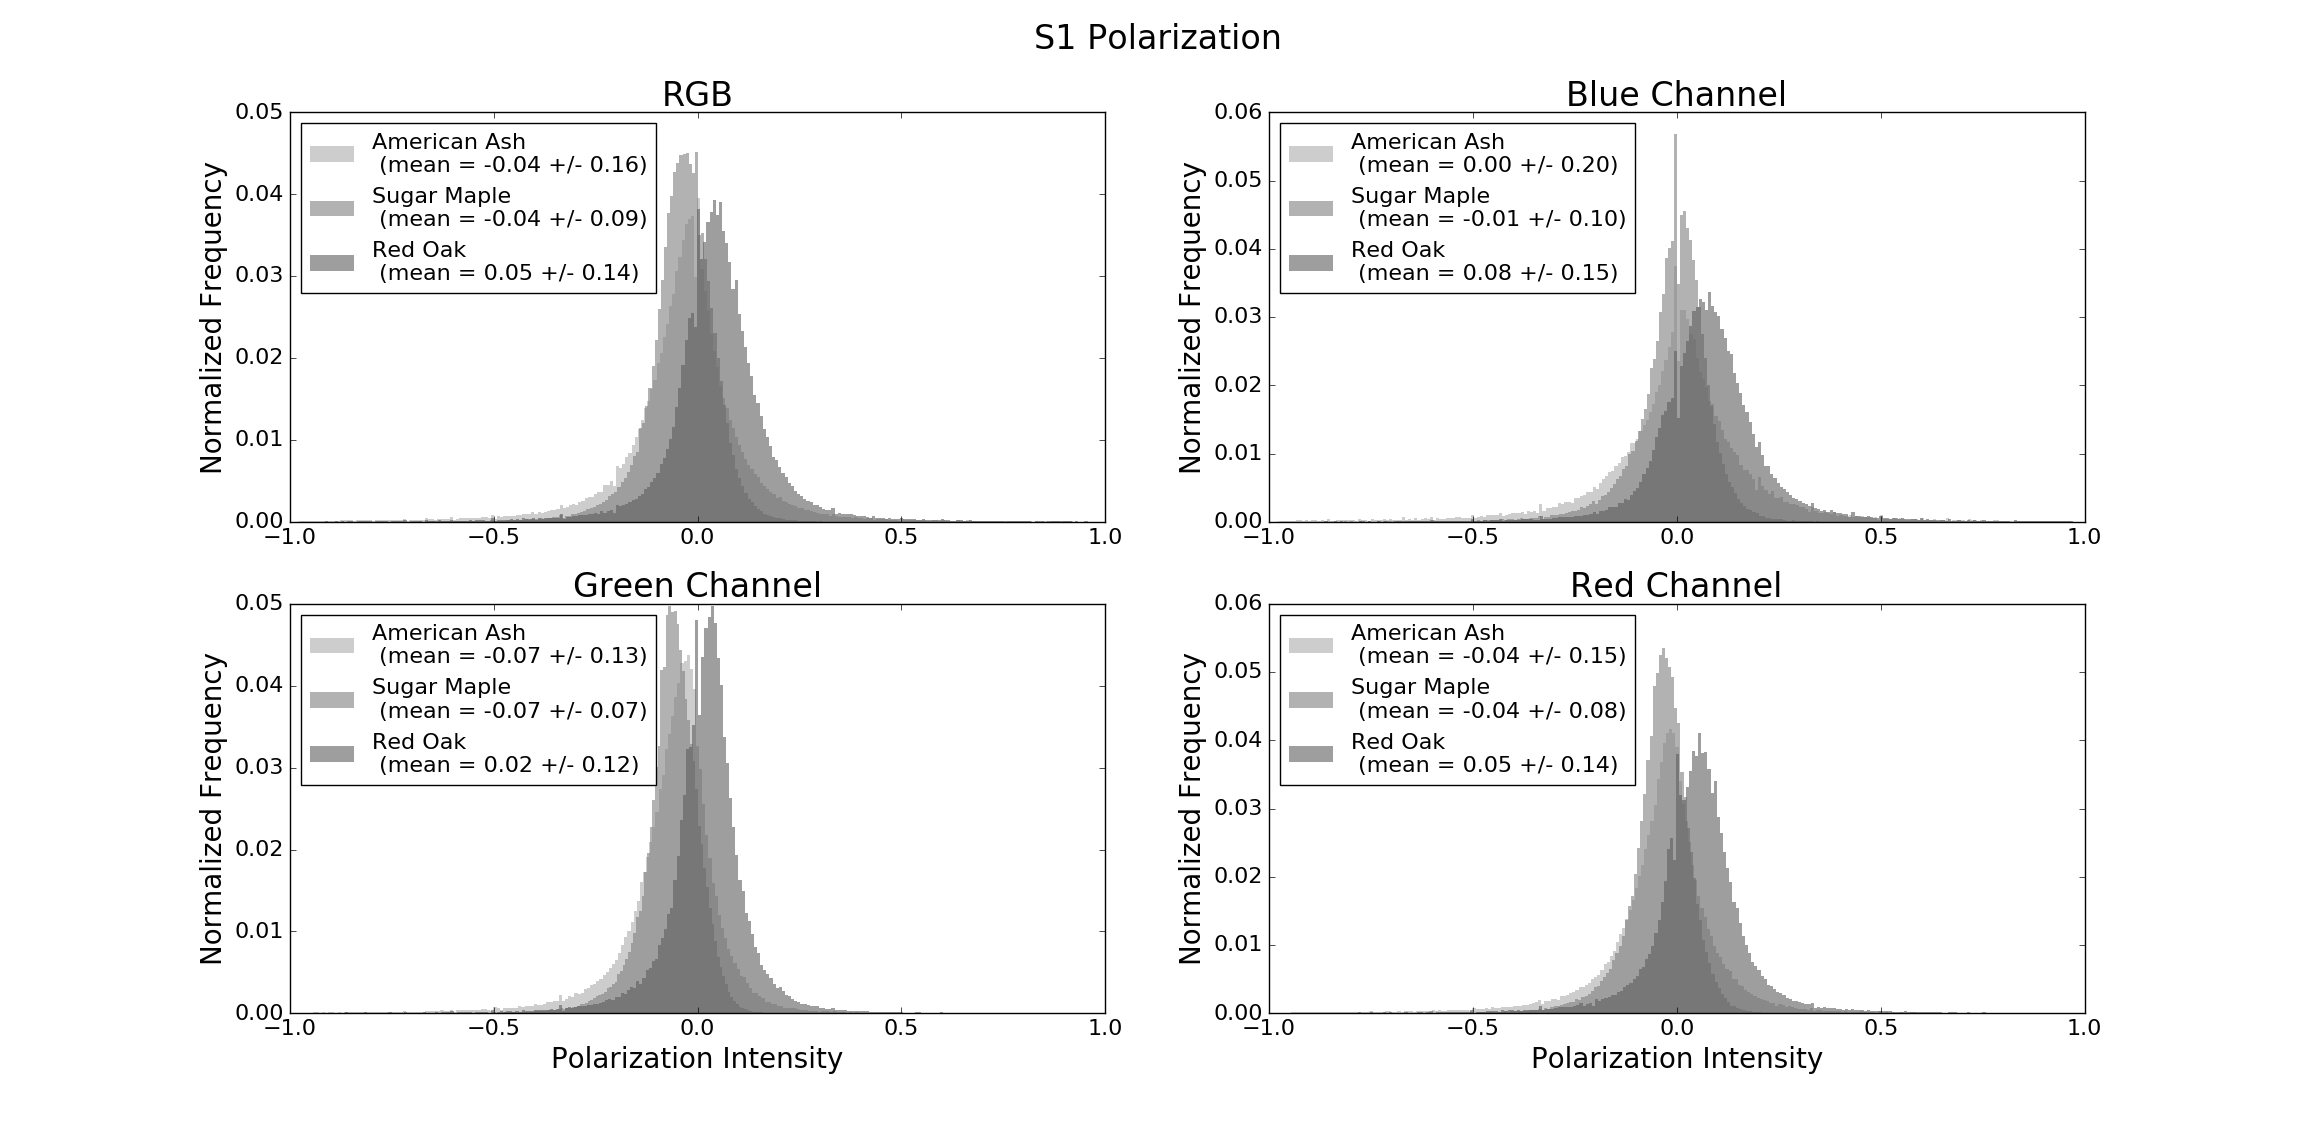
\includegraphics[scale=0.4]{/Sources/Results/7_2_4/S1-polar-v2.png}}
    \end{center}
    \caption{All species, for the diffuse angle of observation 0 week for S1.}
    \label{fig:polarization}
\end{sidewaysfigure}
%
It can be seen that many of the leaves exhibit little to no S1 polarization.  This is expected since much of the S1 polarization results from single scatter surface level phenomena.  The polarization in S2 is shown to be significant.

The polarization can bee seen to be highest in the red and blue where absorption of photons by chlorophyll in the mesophyll layer of the leaf is most prominent.  Structures such as veins may also cause unknown polarization states to result.  Care should be taken when composing images as to what structures are desired for inspection.

The distribution between species in S2 are distributed around different means and variances are as shown in Figure 7.13.
%
\begin{sidewaysfigure}
    \begin{center}
        \makebox[\textwidth]{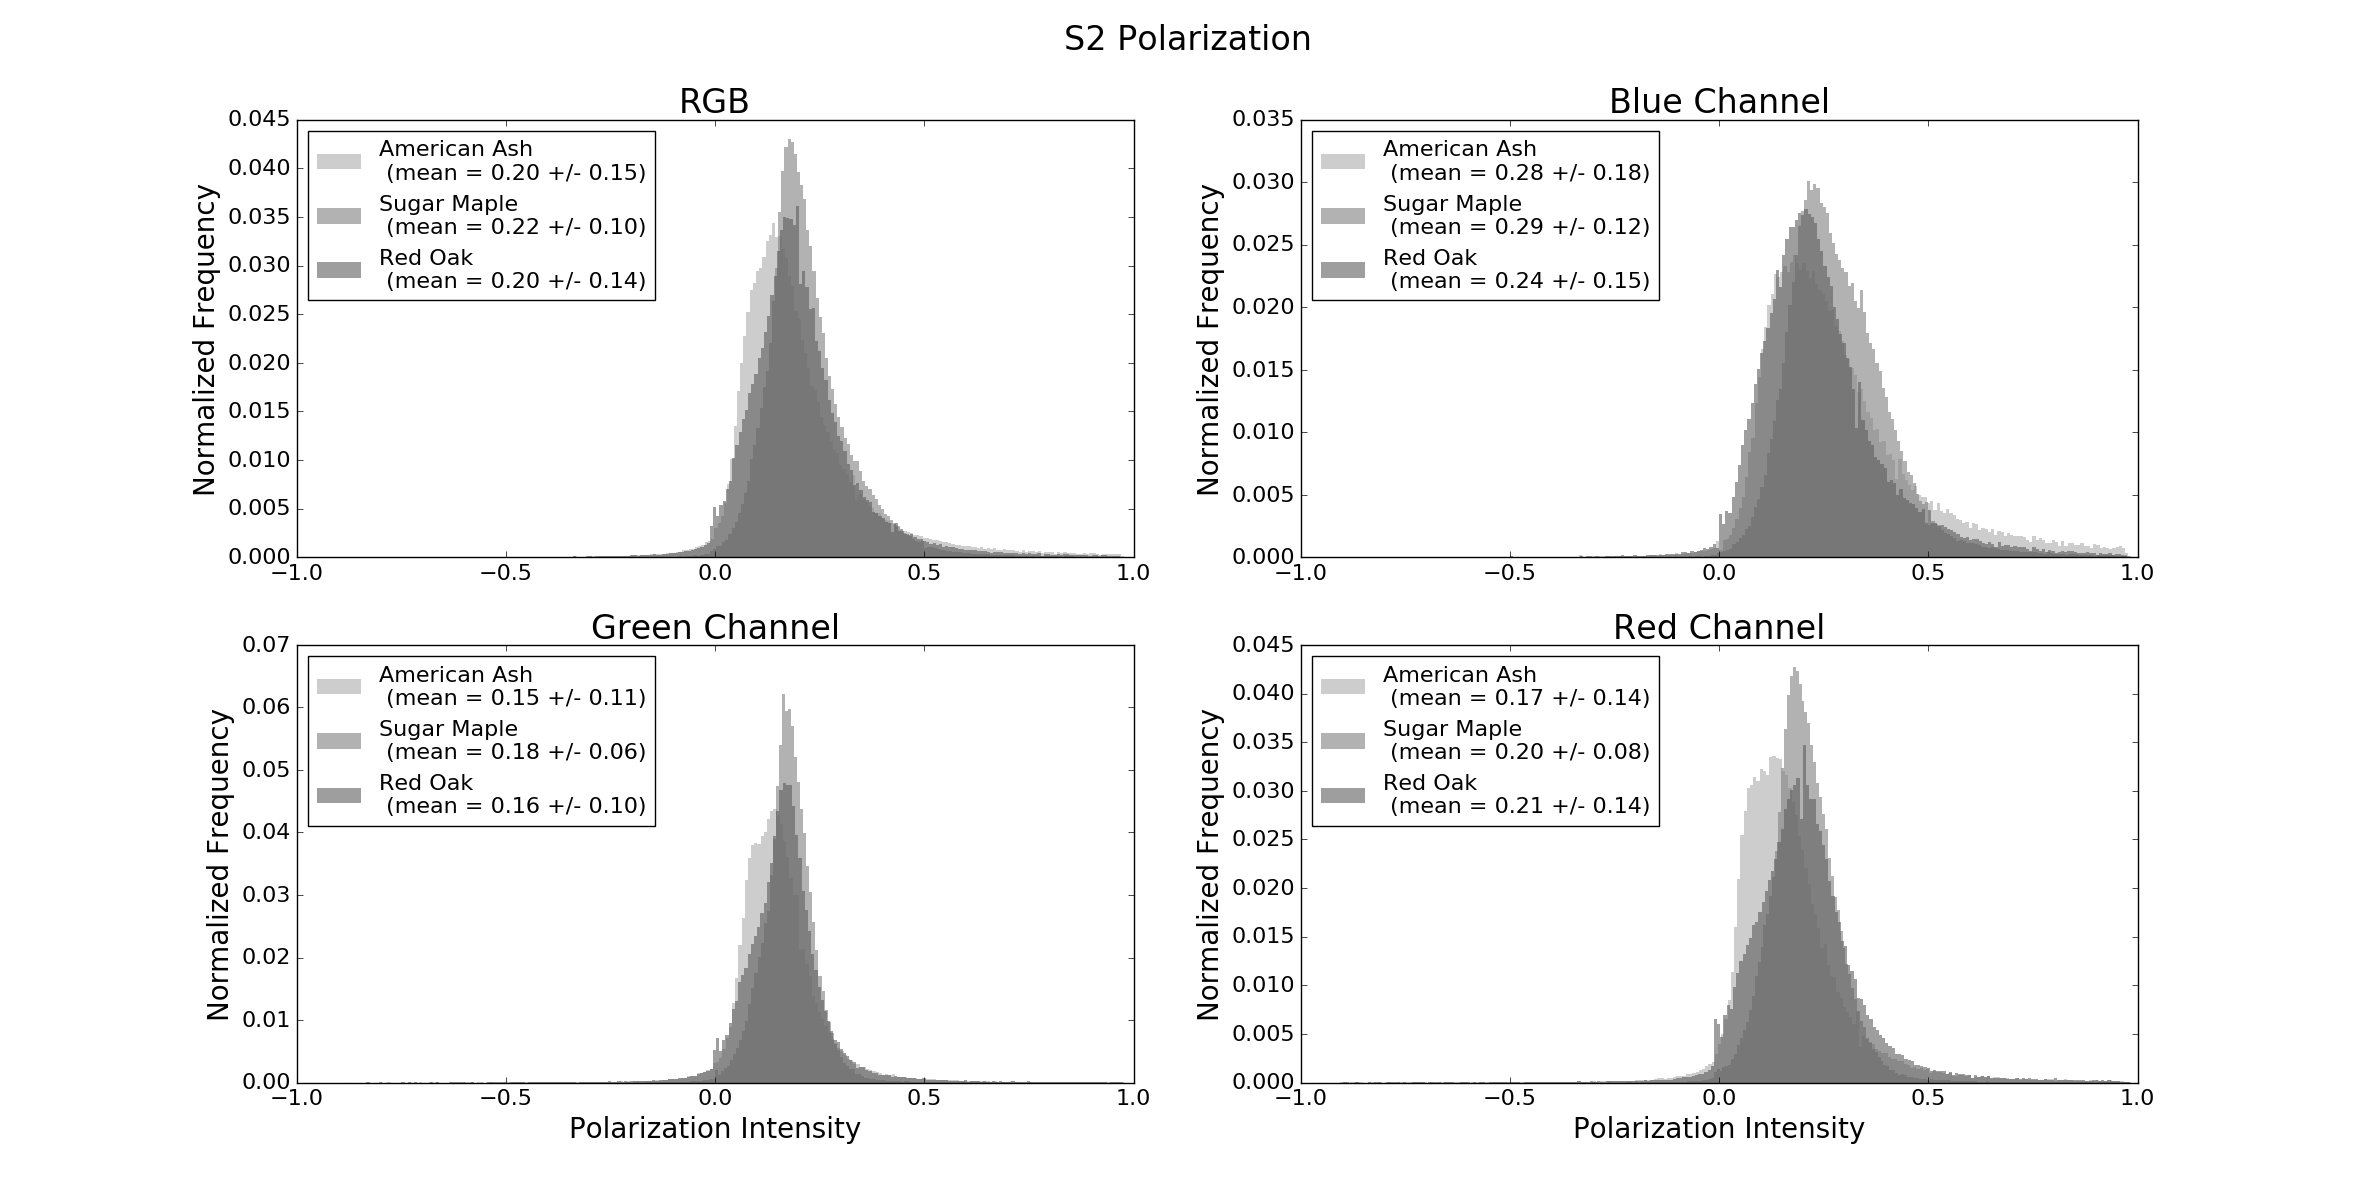
\includegraphics[scale=0.4]{/Sources/Results/7_2_4/S2_polar_v2.png}}
    \end{center}
    \caption{Polarization for all species in the diffuse direction of observation for S2.}
    \label{fig:polarization}
\end{sidewaysfigure}
%
A GLCM analysis in the diffuse direction for all species shows visually distinct clustering.  GLCM dissimilarity and correlation for diffuse scattering can be found in Figure 7.14.
%
\begin{figure}
    \begin{center}
        \makebox[\textwidth]{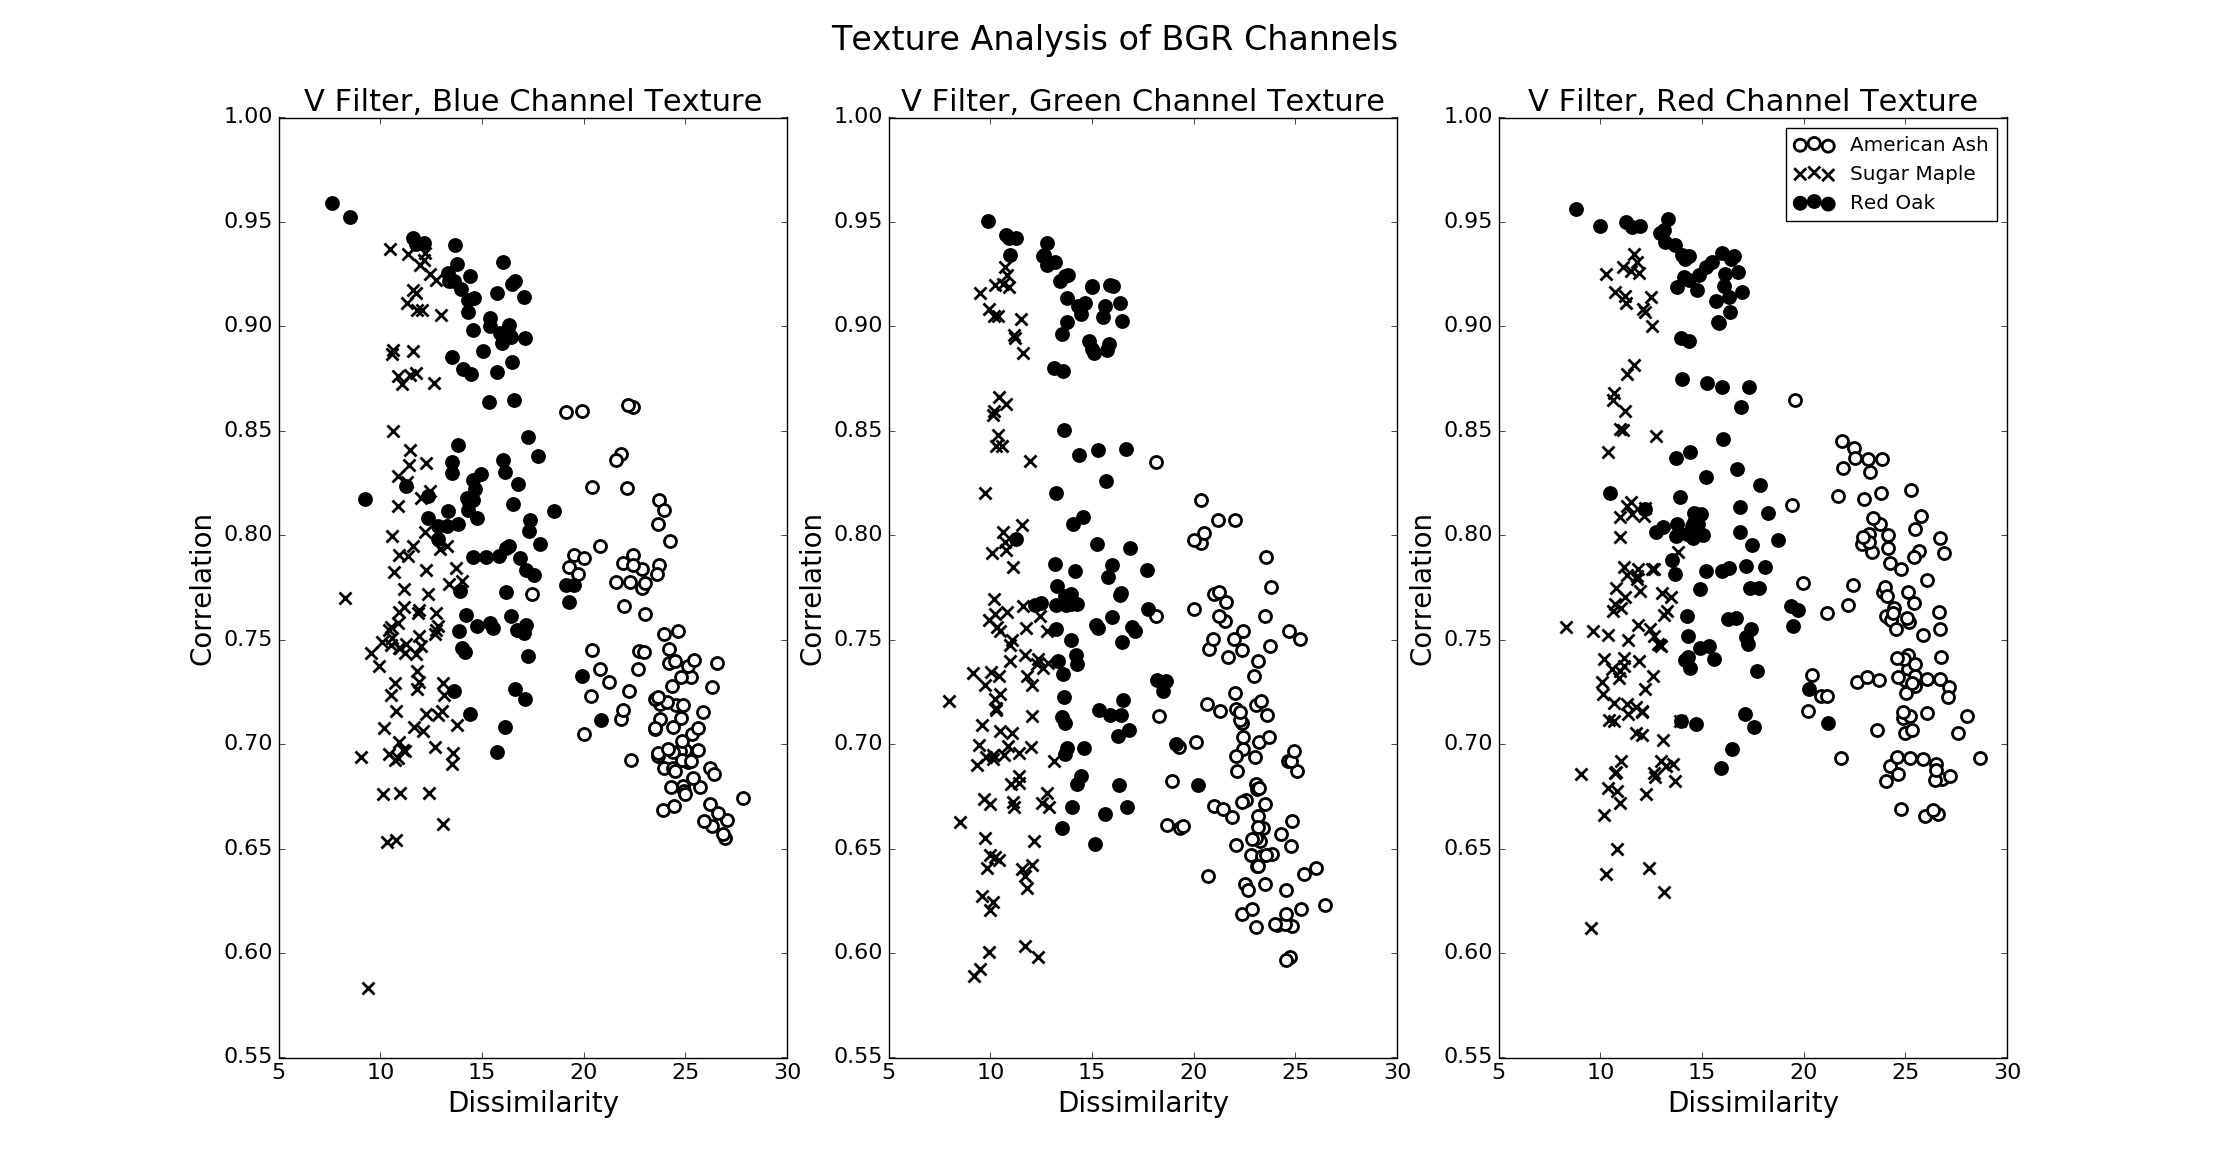
\includegraphics[scale=0.375]{/Sources/Results/glcm/diffuse/V-filter-all-species-rgb-diffuse.png}}
    \end{center}
    \caption{V filter GLCM dissimilarity and correlation for all species in diffuse direction 0 weeks.}
    \label{fig:polarization}
\end{figure}
%
\subsection{Diffuse Leaf Decomposition}
As the breakdown of the leaf occurs, fewer photons are utilized for photosynthesis.  This results in fewer type B photon interactions as the leaves becomes more reflective.  The diffuse portion of the fresh leaf contains a large amount of type B and C photons.  Intricate structures can be seen in the leaf not seen in the specular images since the diffuse light does not oversaturate the sensor.
%
\begin{figure}[htp]
    \centering
    \hspace*{\fill}%
    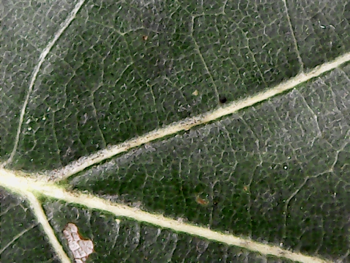
\includegraphics[width=.3\textwidth]{/Sources/Results/7_2_5/oak-0.png}\hfill%
    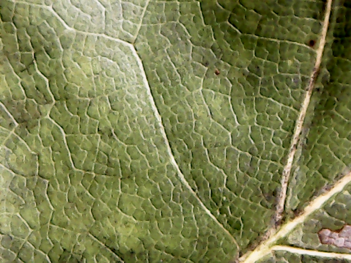
\includegraphics[width=.3\textwidth]{/Sources/Results/7_2_5/red-oak-1.png}
    \hspace*{\fill}%
    \caption{From left to right: Red Oak Freshly Removed and After One Week}
    \label{fig:specular-raw-decompose}
\end{figure}
%
The images above show that in the diffuse direction for Red Oak freshly removed, there are numerous micro segmentations on the leaf surface that were not evident in the specular direction.  These complex wax structures increase the amount of multiple scattering.  As the leaf decomposes, the micro segmentations become less evident as the larger structures become the most prevalent feature on the surface.

Figure 7.16 and Figure 7.17 show's the S1 and S2 polarization in the diffuse direction for a Red Oak leaf as it undergoes the decomposition.
%
\begin{sidewaysfigure}
    \begin{center}
        \makebox[\textwidth]{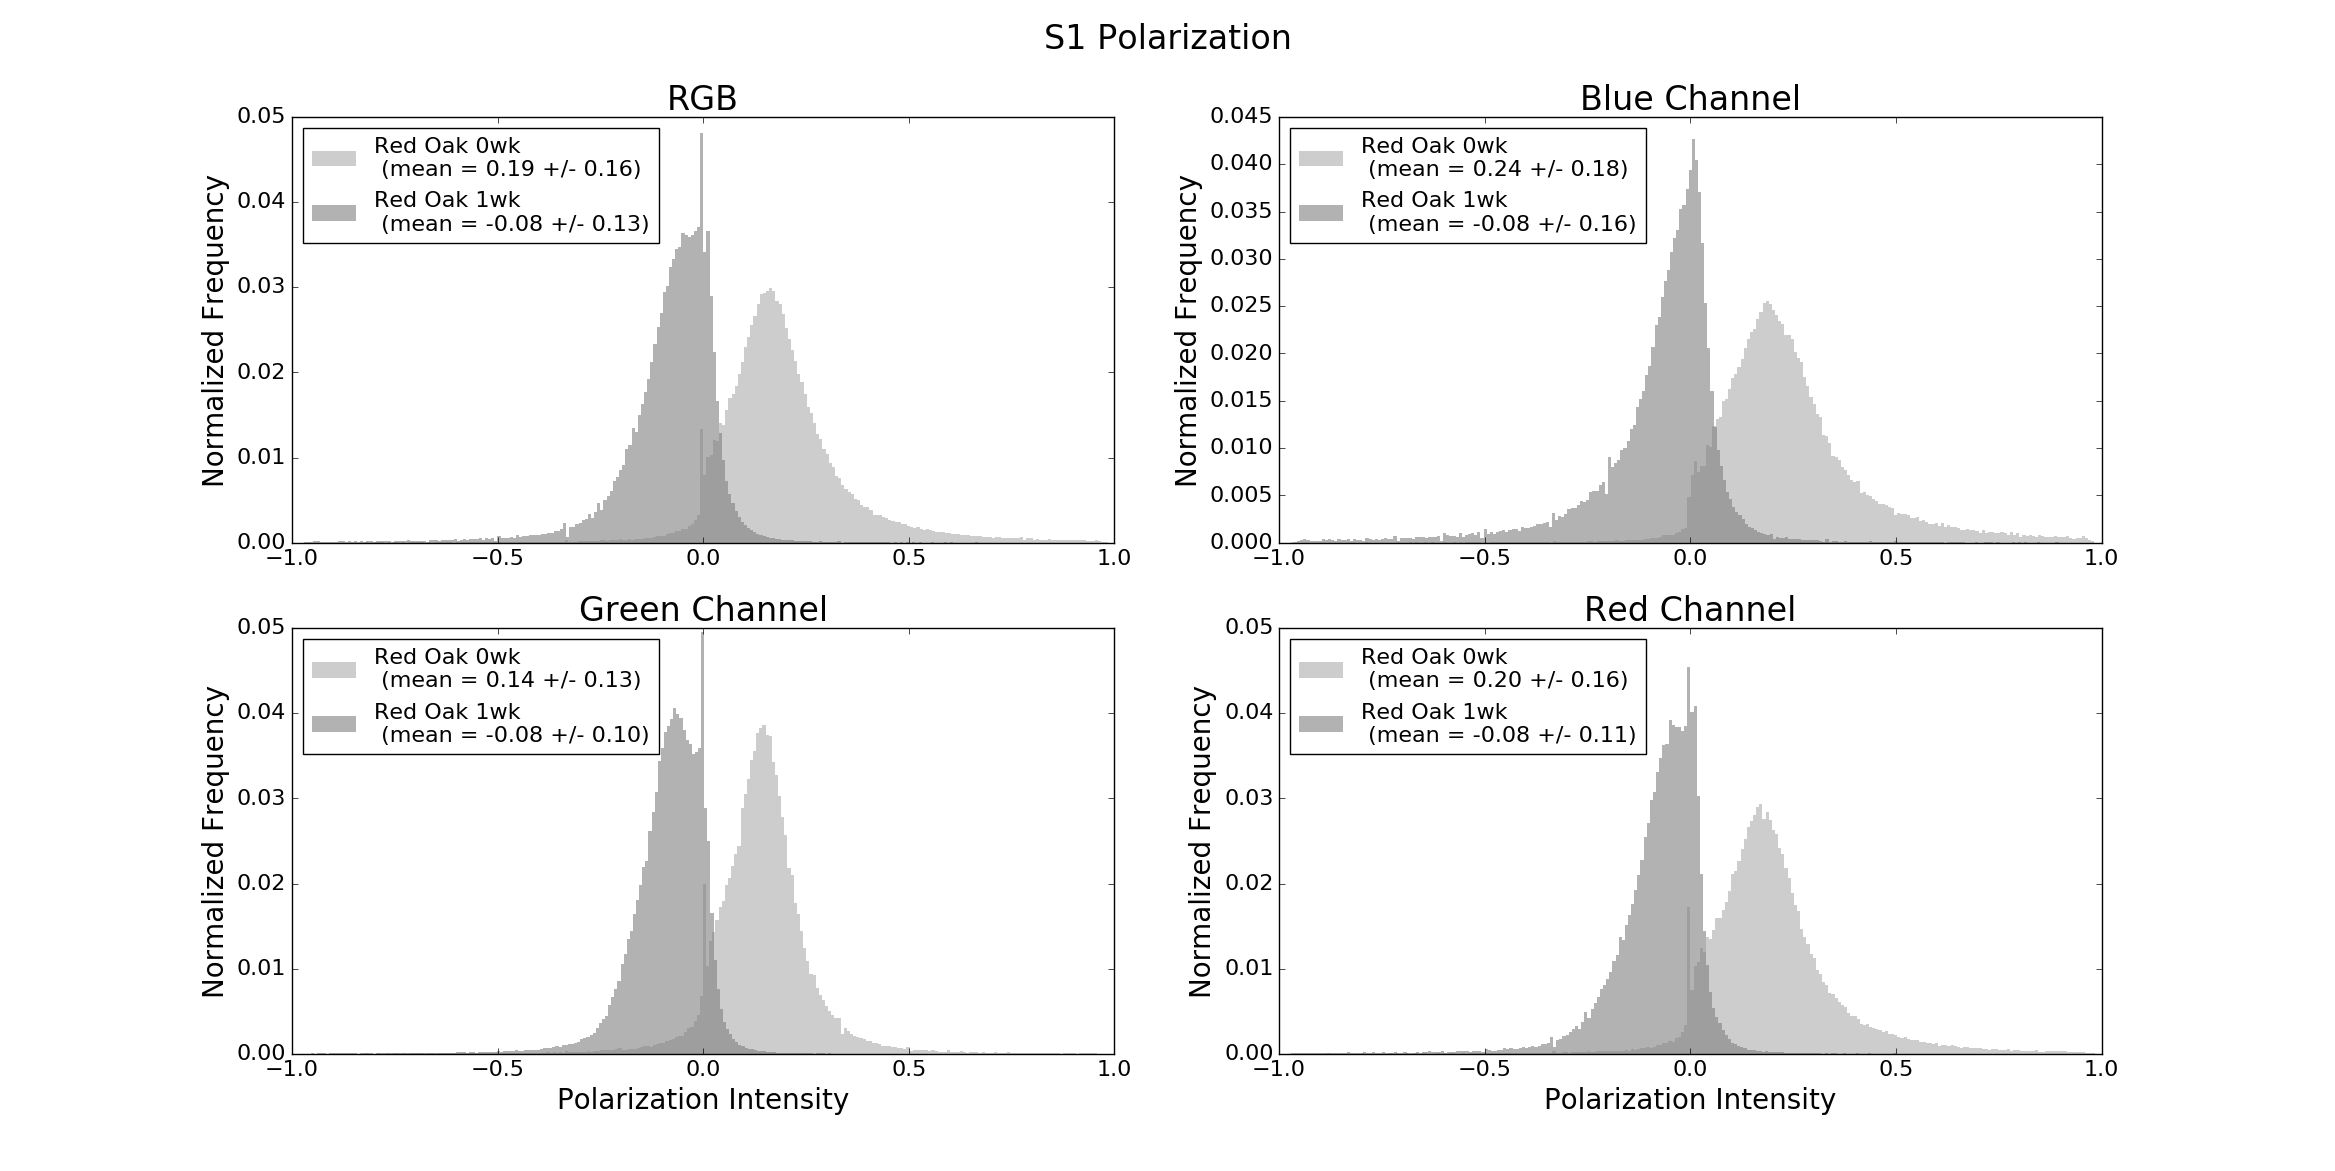
\includegraphics[scale=0.4]{/Sources/Results/7_2_5/S1-polar-v2.png}}
    \end{center}
    \caption{Red Oak in the diffuse direction for S1}
    \label{fig:polarization}
\end{sidewaysfigure}
%
The S1 polarization component is low for both the fresh and decomposing leaf in the diffuse direction.  Most of the polarization that results is not purely perpendicular or parallel to the incident surface.  The S and P component of polarization are mostly cancelled out.
%
\begin{sidewaysfigure}
    \begin{center}
        \makebox[\textwidth]{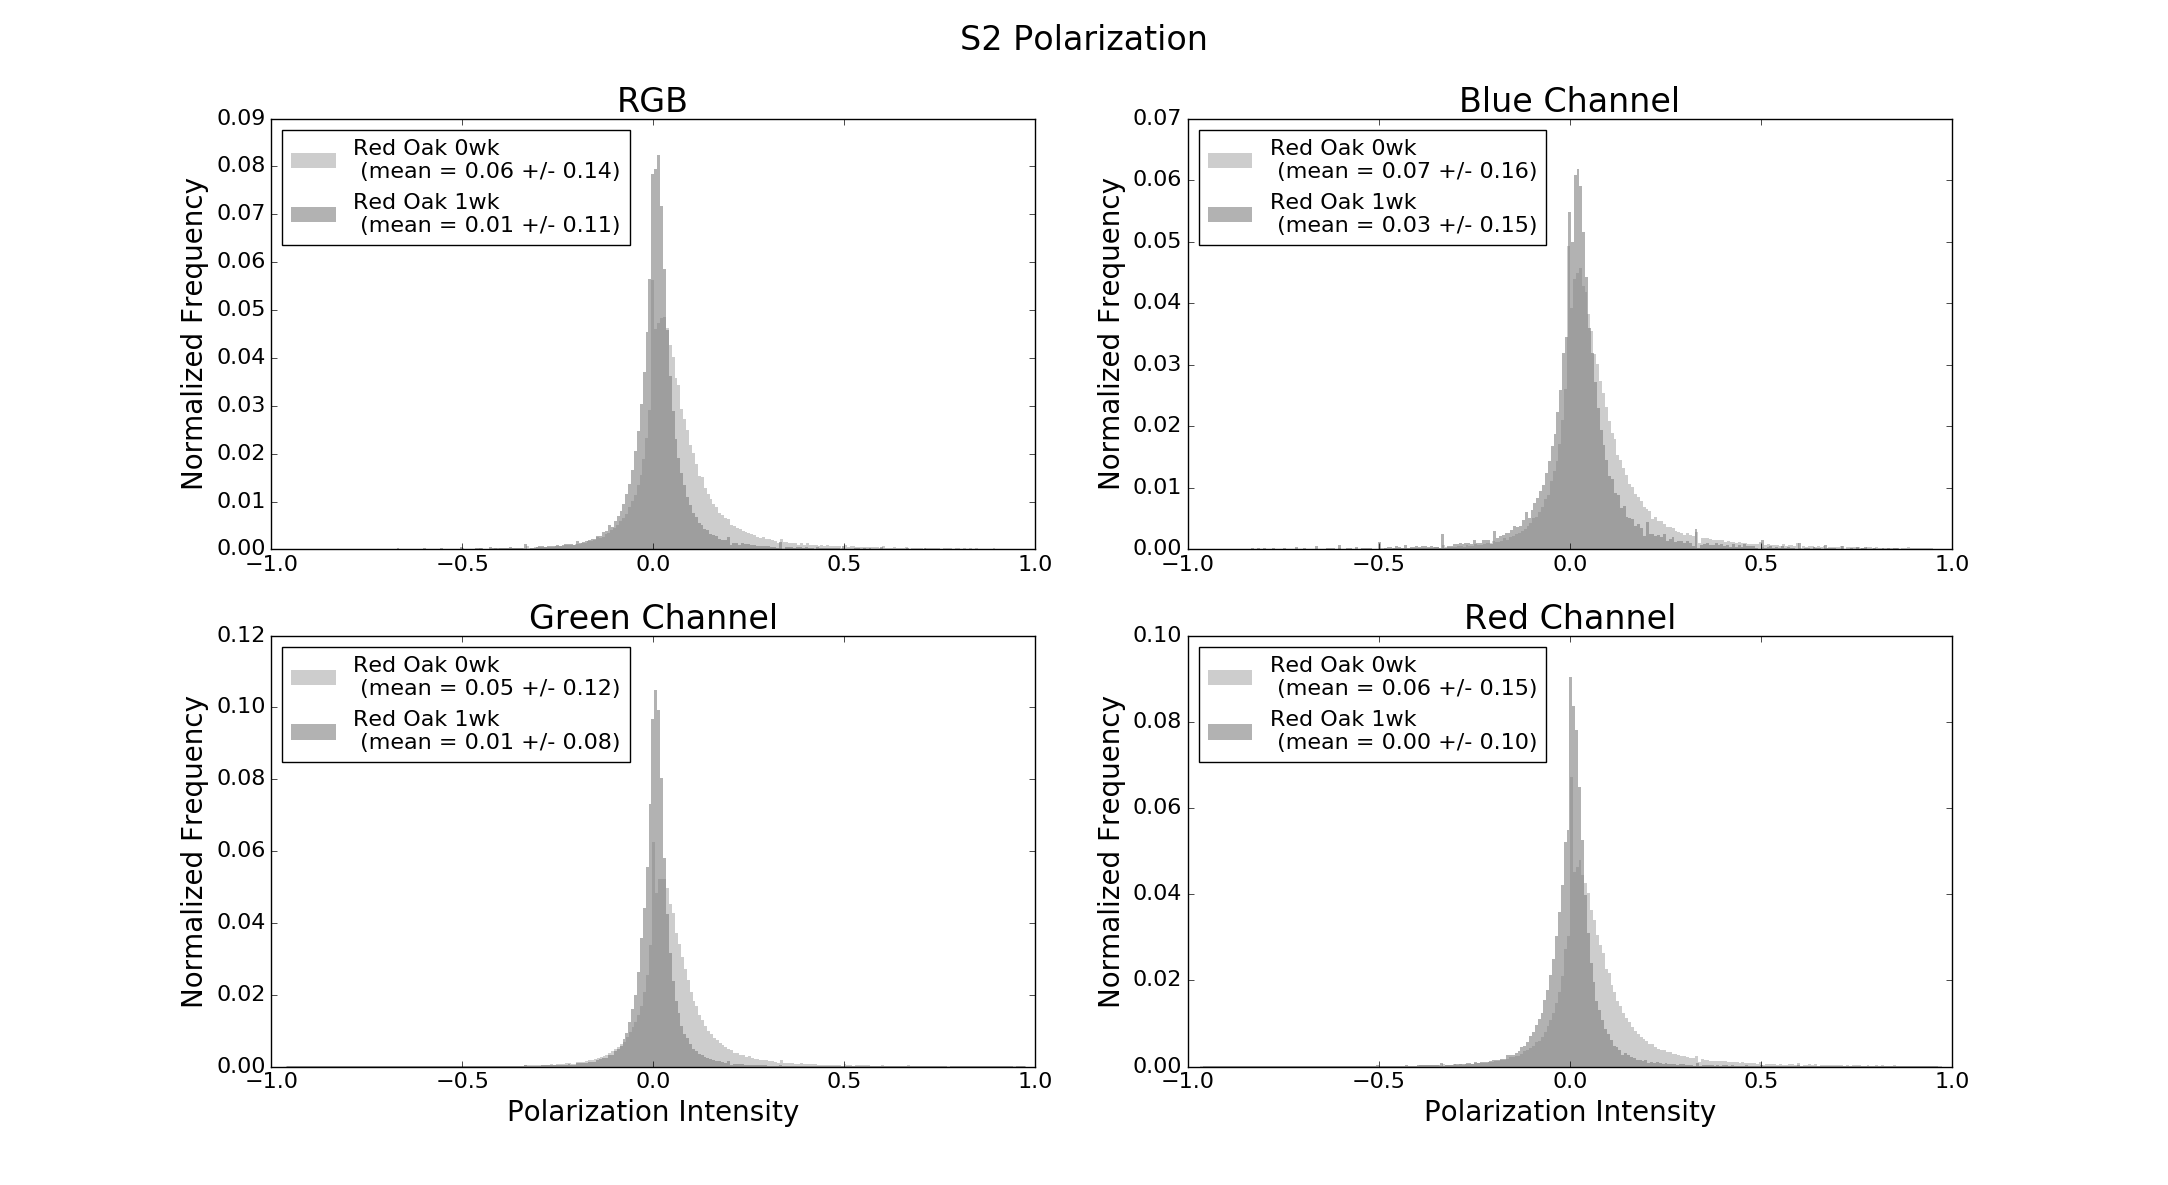
\includegraphics[scale=0.4]{/Sources/Results/7_2_5/S2-polar_v2.png}}
    \end{center}
    \caption{Red Oak in the diffuse direction for S2}
    \label{fig:polarization}
\end{sidewaysfigure}
%
There is S2 polarization that arises from each specimen, and it is shown to be higher for red oak leaves that are undergoing the process of decomposition.

As the composition of a leaf changes, more polarization results as an effect of the physiological breakdown causes less absorption and more volume scattering.  Although diffuse surfaces are supposed to create equal amounts of randomized polarized states, resulting in no overall polarization, it is shown here that in some cases the diffuse portion is polarized, especially in the S2 component.  This information could potentially be useful for determining physiological properties of leaves.

The GLCM in the diffuse direction shows that as the wax structure becomes less filled with water and decompresses, the surface of the leaf appears smoother, since there is less noise caused by multiple scattering through the thicker wax cuticle of the fresh leaves.  The result is that healthier leaves create more dissimilarity for the captured images.  This is shown in Figure 7.18.
%
\begin{figure}
    \begin{center}
        \makebox[\textwidth]{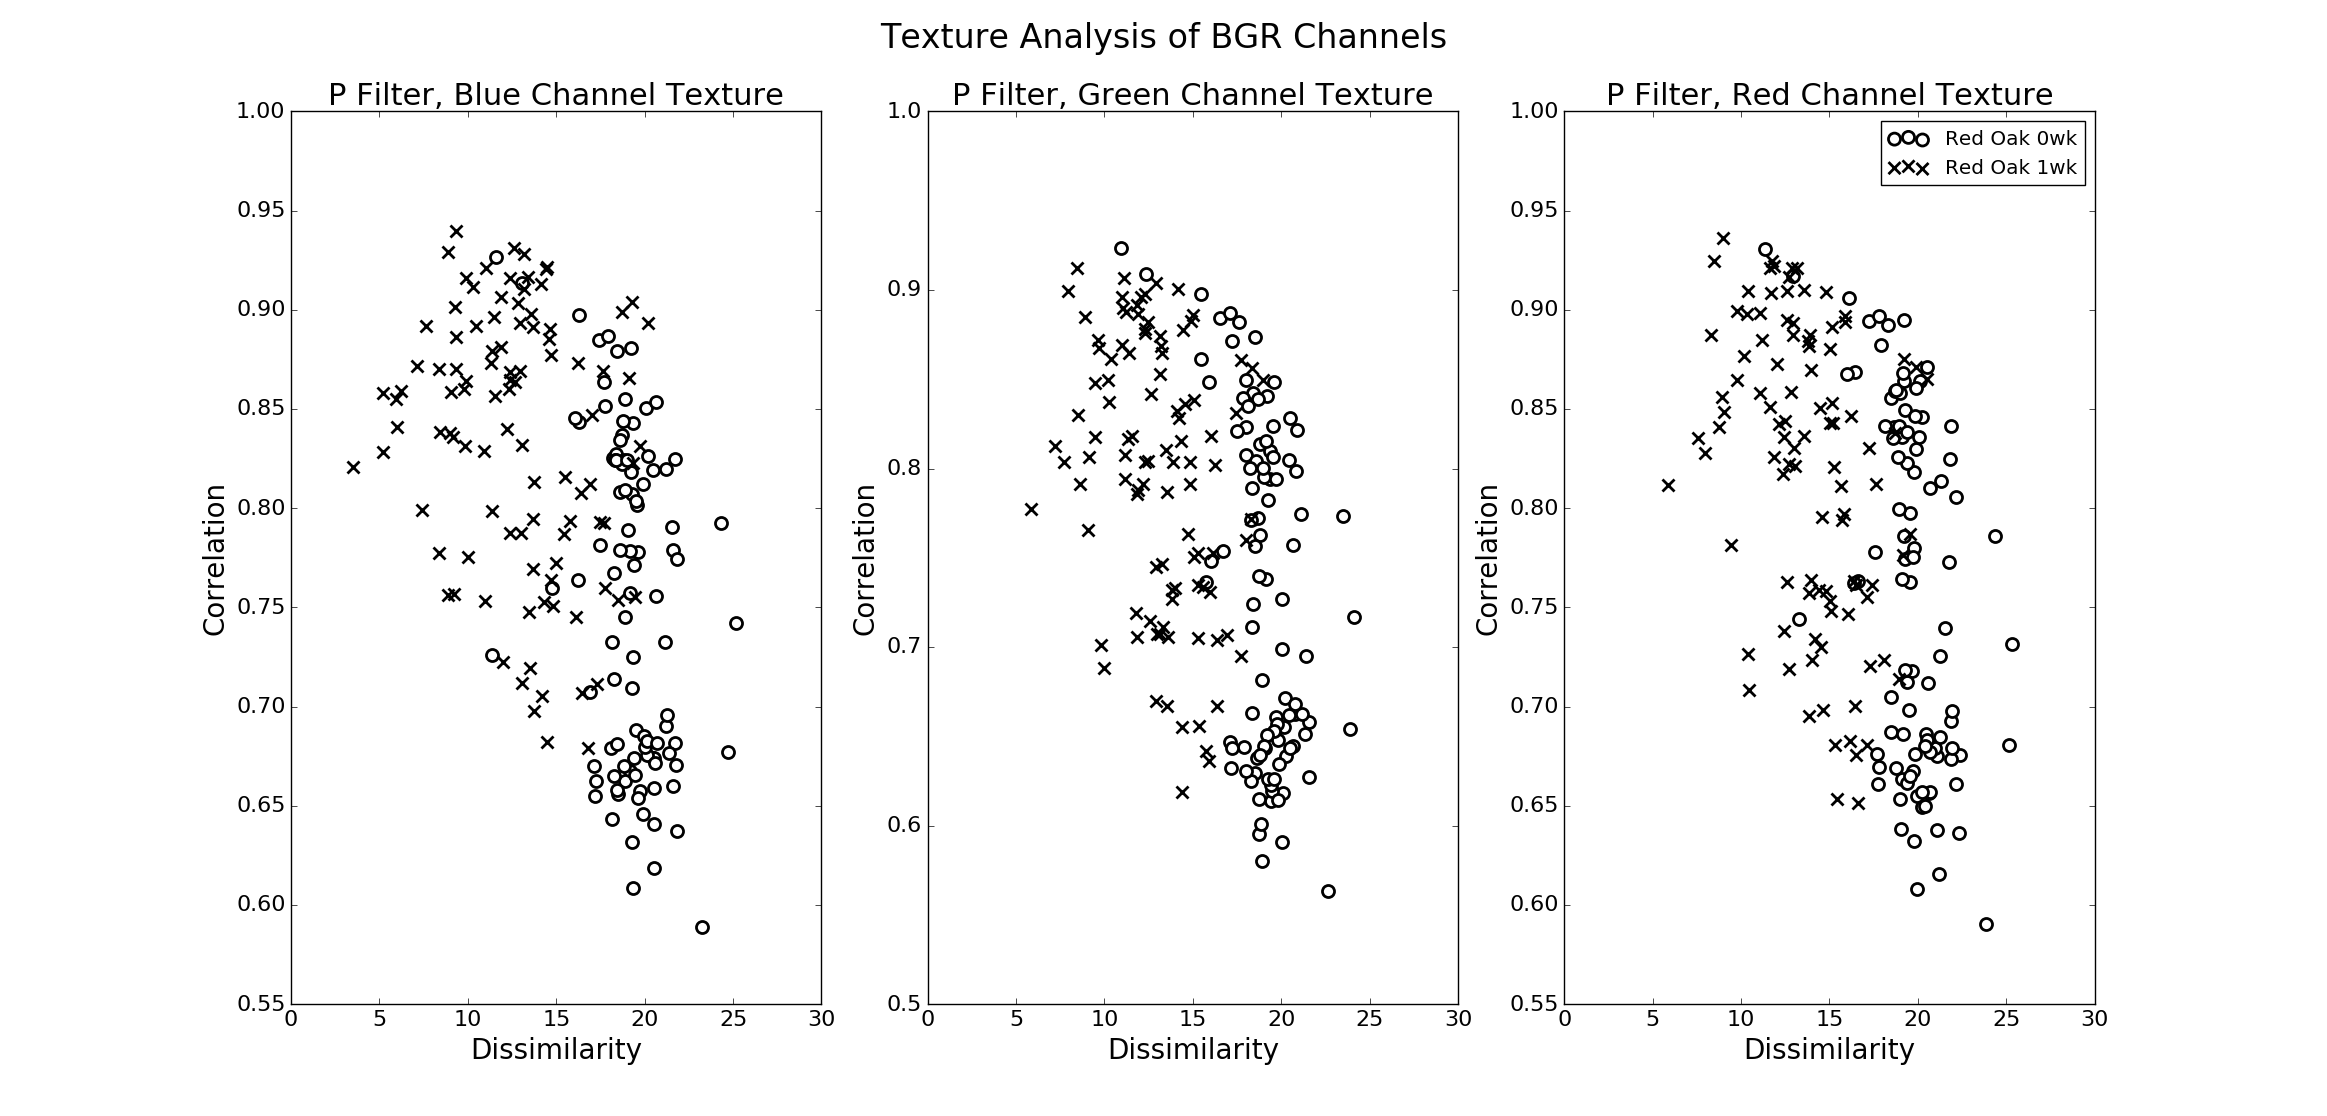
\includegraphics[scale=0.375]{/Sources/Results/glcm/diffuse/0wk-1wk-P-filter-red-oak-rgb-diffuse.png}}
    \end{center}
    \caption{P filter GLCM dissimilarity and contrast in diffuse direction for red oak 0 week vs 1 week}
    \label{fig:polarization}
\end{figure}
%
The multiple scattering and microstructures evident in the thicker wax of a freshly removed oak leaf creates a high amount of dissimilarity and lower correlation than after a week of drying.

\subsection{Diffuse Classification Results}
Support vector classification was performed on all leaves collected for each of the species with zero and one week combined in order to show the ability to classify similar species even if interclass variance exists.  Overall the diffuse results were slightly less accurate than the specular results, but this may be due to the overall noise in the diffuse images acquired.  Further investigation is required in this regard.

The confusion matrix shows that ash is the most correctly identified class, with the highest precision and recall when compared to other classes.  Classification precision for oak and maple were similar.

The learning curve shows good results as more samples are added, but towards the end shows the score decreases slightly.  Additional samples should be investigated to ensure the validity of this model.

Overall the model does show correlation between each species texture and polarization characteristics.  This is indicated by high accuracy in classification as shown by the confusion matrix and the precision scores seen in Table 7.4.
%
\begin{figure}[!htb]
    \begin{center}
        \makebox[\textwidth]{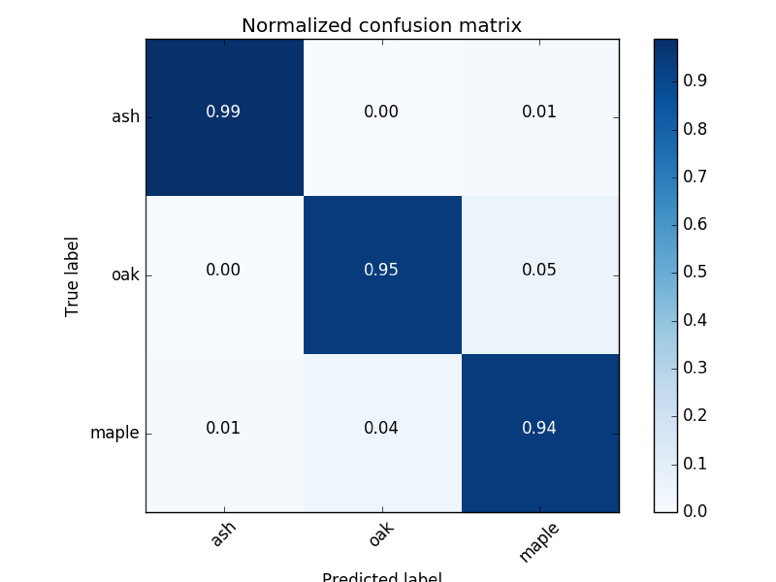
\includegraphics[scale=0.9]{/Sources/Results/7_2_6/confusion.png}}
    \end{center}
    \caption{Confusion matrix for all species observed in the diffuse direction.}
    \label{fig:polarization}
\end{figure}
%
%
\begin{figure}[!htb]
    \begin{center}
        \makebox[\textwidth]{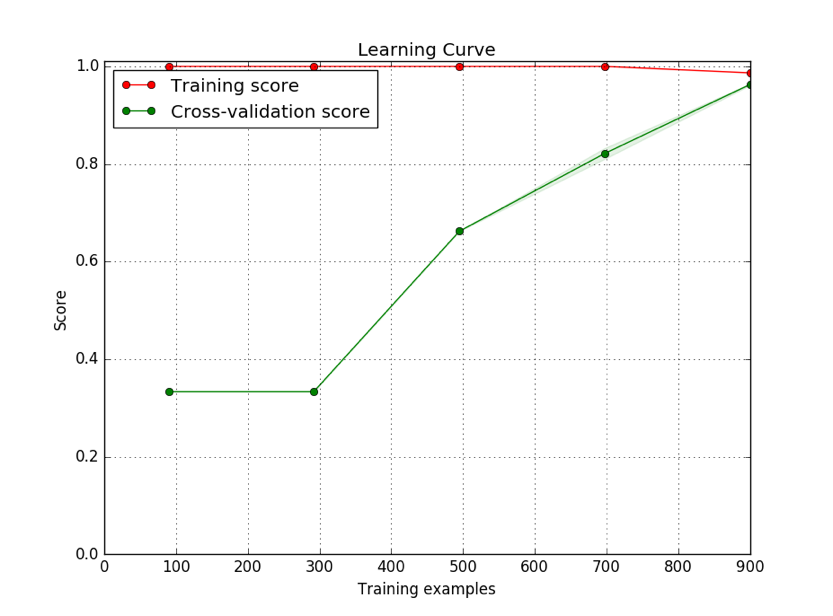
\includegraphics[scale=0.9]{/Sources/Results/7_2_6/learning_curve.png}}
    \end{center}
    \caption{Learning curve for All species observed in the diffuse direction}
    \label{fig:polarization}
\end{figure}
%
%
\begin{table}[htb]
  \centering
  \begin{tabular}{lllll}
    \toprule
    \textbf{Class} & \textbf{Precision} & \textbf{Recall} & \textbf{F1 Score} & \textbf{Support} \\
    \midrule
      \texttt{0.0} & 0.98 & 0.99 & 0.99 & 600 \\
      \texttt{1.0} & 0.93 & 0.94 & 0.94 & 600 \\
      \texttt{2.0} & 0.93 & 0.92 & 0.93 & 600 \\
      \texttt{avg/total} & 0.95 & 0.95 & 0.95 & 1800 \\
    \bottomrule
  \end{tabular}
  \caption{%
    Scores for Classification in the Diffuse Direction with Polarization and Texture in Diffuse Direction.
  }
  \label{tab:Packages}
\end{table}
\begin{table}[htb]
  \centering
  \begin{tabular}{lllll}
    \toprule
    \textbf{Class} & \textbf{Precision} & \textbf{Recall} & \textbf{F1 Score} & Support\\
    \midrule
      \texttt{0.0} & 0.94 & 0.95 & 0.94 & 600 \\
      \texttt{1.0} & 0.90 & 0.92 & 0.91 & 600 \\
      \texttt{2.0} & 0.89 & 0.86 & 0.88 & 600 \\
      \texttt{avg/total} & 0.91 & 0.91 & 0.91 & 1800 \\
    \bottomrule
  \end{tabular}
  \caption{%
    Scores for Classification in the Diffuse Direction with Just Polarization in Diffuse Direction.
  }
  \label{tab:Packages}
\end{table}
%
\begin{table}[htb]
  \centering
  \begin{tabular}{lllll}
    \toprule
    \textbf{Class} & \textbf{Precision} & \textbf{Recall} & \textbf{F1 Score} & Support\\
    \midrule
      \texttt{0.0} & 0.98 & 0.99 & 0.99 & 600 \\
      \texttt{1.0} & 0.77 & 0.85 & 0.81 & 600 \\
      \texttt{2.0} & 0.84 & 0.74 & 0.79 & 600 \\
      \texttt{avg/total} & 0.86 & 0.86 & 0.86 & 1800 \\
    \bottomrule
  \end{tabular}
  \caption{%
    Scores for Classification in the Diffuse Direction with Just Texture in Diffuse Direction.
  }
  \label{tab:Packages}
\end{table}
%
Comparison of with the use of in Table limited feature sets, shows again that texture combined with polarization returns better results than if only one were used.  Overall classification in the diffuse direction was slightly less accurate than that of our specular measurements.

In the future principal component analysis should be utilized to isolate the top parameters for each group in order to eliminate any bias that is caused from there being more polarization features than texture features. An additional image should be acquired with no polarization filter in place, to represent $S_0$ and create a better mark for texture feature only comparison.

\section{Regression}
Previous results show that classification between species can be performed with high levels of accuracy even if a large amount of interclass variance exists due to varying physiological states of each leaf.  Therefore, investigation into acquiring more accurate measures as to the plants' current physiological state, such as water and pigment concentration, would be useful for a more detailed explanation of previous results.

Determining the relationship between the relative water content of a plant's leaf, versus features extracted from images taken in the visible portion of the spectrum with a camera, requires data to be fit in a regression model.  Support Vector Regression (SVR) is an extension of linear regression with the purpose of minimizing the distance of each point to the best fit line.

The y dependent variable was determined by measuring the relative water content of the Devils Ivy plant using the procedure previously described.  Samples were extracted from each polarization filter for the purpose of GLCM analysis.  The average dissimilarity, contrast, energy and correlation of 100 samples randomly selected from the entire image were utilized to quantify the texture of each individual leaf at different levels of RWC.  The S1 and S2 polarizance parameters were also calculated for each individual pixel. Each pixel was binned together to create histograms for S1 and S2.  The probabilities for 20 bins ranging from -1 to 1 were utilized to determine the polarization component of each sample.

Principal component analysis was utilized to extract the most useful features for plotting against the RWC.  The principal component can be seen plotted against RWC for the specular case in Figure 7.21.
%
\begin{figure}[!htb]
    \begin{center}
        \makebox[\textwidth]{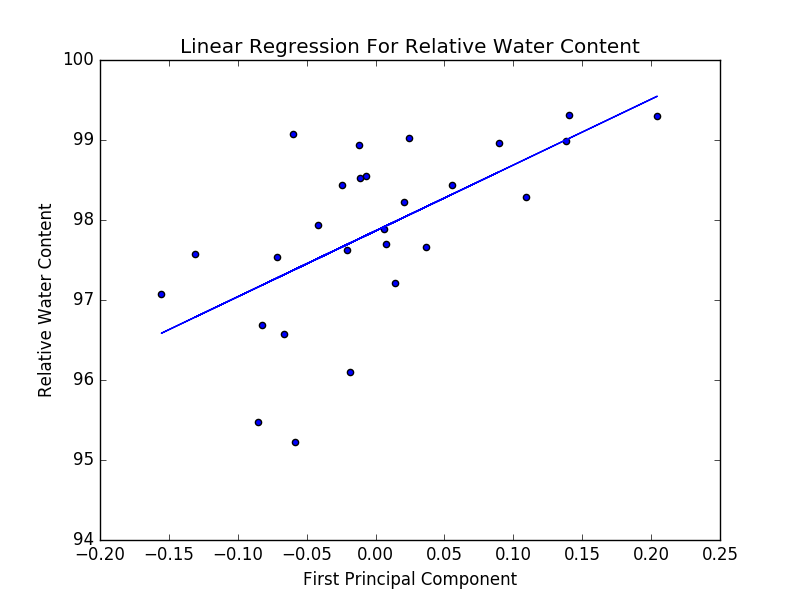
\includegraphics[scale=0.65]{/Sources/Results/rwc-regression.png}}
    \end{center}
    \caption{Linear Regression for RWC and 1st principal component - Specular}
    \label{fig:polarization}
\end{figure}
%
%
\begin{table}[htb]
  \centering
  \begin{tabular}{ll}
    \toprule
    \textbf{Metric} & \textbf{Score}\\
    \midrule
      \texttt{r2} & 0.376 \\
      \texttt{RMS} & 0.758 \\
    \bottomrule
  \end{tabular}
  \caption{%
    Scores for Regression in the Specular Direction
  }
  \label{tab:Packages}
\end{table}
%
Analyzing the specular polarization and extracting texture features showed high levels of correlation for biological regression problems with an $r^2$ of 0.376.  The classifier was cross validated using K-fold validation with 10 folds.  The performance of the classifier is summarized in Table.
The root mean squared shows the accuracy to be within 0.5% of the actual value for the predicted linear model. Further data is required to more accurately fit this model, although the initial results are promising.
%
The diffuse direction did not have as much usefulness in determining the RWC for the data that was acquired and tested.  The $r^2$ value was nearly zero, meaning the $Y$ values could not be explained by the input $X$ variables for the linear relationship tested. Figure 7.22 shows this poor relationship.  Further analysis and data reduction techniques could be applied to further analysis any potential relationship between texture, polarization and relative water content.
\begin{figure}[!htb]
    \begin{center}
        \makebox[\textwidth]{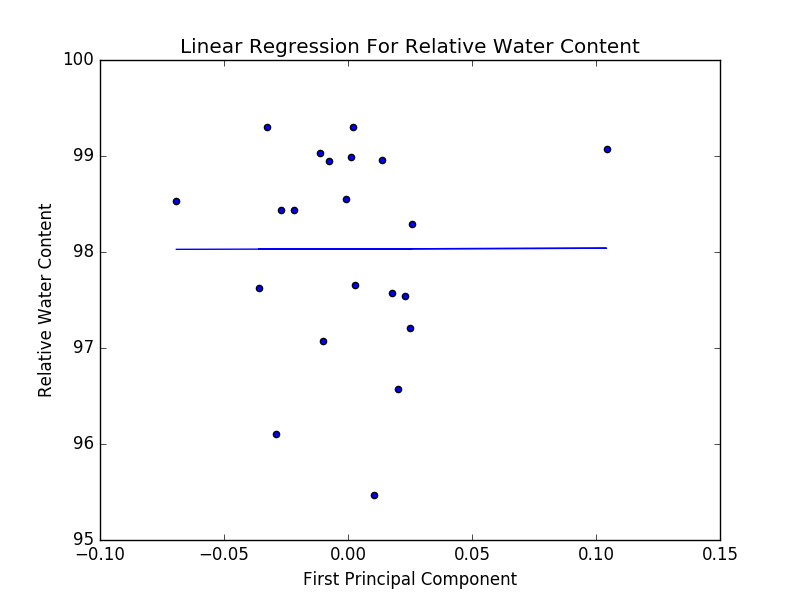
\includegraphics[scale=0.65]{/Sources/Results/rwc-diffuse.png}}
    \end{center}
    \caption{Linear Regression for RWC and 1st principal component - Diffuse}
    \label{fig:polarization}
\end{figure}
%
%
\begin{table}[htb]
  \centering
  \begin{tabular}{ll}
    \toprule
    \textbf{Metric} & \textbf{Score}\\
    \midrule
      \texttt{r2} & 4.178e-06 \\
      \texttt{RMS} & 1.126 \\
    \bottomrule
  \end{tabular}
  \caption{%
    Scores for Regression in the Diffuse Direction
  }
  \label{tab:Packages}
\end{table}
